% !TEX encoding = UTF-8
% !TEX TS-program = pdflatex
% !TEX root = ../tesi.tex

%**************************************************************
\chapter{Progettazione}
\label{cap:progettazione}

La progettazione nel caso del prodotto che ho dovuto sviluppare si è concentrata particolarmente sulla piattaforma di api.ai, in quanto rappresentava la maggior parte del lavoro. Successivamente sono passato alla progettazione delle classi da introdurre nel codice già creato dall'azienda, per gestire le nuove funzionalità dei \glspl{Chatbot}.

\section{Studio di api.ai}
Prima di passare all'attività di progettazione è stato fondamentale analizzare e studiare a fondo le possibilità che api.ai mette a disposizione per la creazione del prodotto a me richiesto. I concetti base per capire il funzionamento di api.ai sono quattro:
\begin{itemize}
	\item \textbf{agent}: gli \emph{agents} sono meglio descritti come moduli NLU (Natural Language Understanding). Questi possono essere inclusi nell'applicazione, nel prodotto o nel servizio e trasformano le richieste di utenti naturali in dati attivi. Questa trasformazione si verifica quando un input utente corrisponde a uno degli \emph{intent} all'interno dell'\emph{agent};
	\item \textbf{intent}: sono una mappatura tra quello che l'utente può scrivere in input e l'azione che il software deve intraprendere. Un \emph{intent} è formato dalle seguenti sezioni:
	\begin{itemize}
		\item\textbf{ \emph{user says}}: perché l'\emph{agent} capisca la domanda, sono necessari esempi di come la stessa domanda può essere posta in modi diversi. Lo sviluppatore aggiunge queste permutazioni alla sezione \emph{user says} dell'\emph{intent}. Più variazioni vengono aggiunte all'\emph{intent}, meglio l'\emph{agent} comprenderà l'utente;
		\item \textbf{\emph{action}}: contiene il nome della \emph{action}, che può essere utilizzato per attivare una particolare funzione del prodotto, e la tabella dei \textbf{\emph{parameters}}. I \emph{parameters} possono essere intesi come gli elementi che collegano le parole nelle \emph{user says} alle \emph{entities};
		\item \textbf{\emph{response}}: in questa sezione è possibile definire la risposta di api.ai quando l'\emph{intent} viene attivato. Non è stato quasi mai utilizzato, in quanto la risposta viene generata nella \emph{business logic}.
	\end{itemize}
	\item \textbf{context}: i \emph{context} rappresentano il contesto corrente della richiesta di un utente. Ciò è utile per differenziare frasi che possono essere vaghe o avere significati diversi a seconda delle preferenze dell'utente, della posizione geografica, della pagina corrente di un'applicazione o dell'argomento della conversazione. È possibile impostare un \emph{lifespan} ad ognuno di essi per definire dopo quante richieste il \emph{context} deve scadere;
	\item \textbf{entity}: le entities sono strumenti potenti utilizzati per estrarre i valori dei parametri dagli input degli utenti. Tutti i dati importanti che si desidera ottenere dalla richiesta di un utente, avranno un'entità corrispondente. Le \emph{system entities} sono entità pre-costruite fornite da api.ai per facilitare la gestione dei più comuni concetti (luoghi, orari, colori, ecc..). È possibile poi definire le proprie \emph{entities} in base alle necessità dello sviluppatore;
\end{itemize}


\section{Progettazione agents api.ai}
Durante la progettazione degli \emph{agents} per api.ai è stato necessario definire tutti gli \emph{intents} utili a soddisfare i requisiti definiti durante l'analisi dei requisiti. Il passo successivo è stato quello di progettare le \emph{user says} per ogni \emph{intent} e le relative \emph{entity}.

\subsection{Gestore di eventi}
\subsubsection{Intent}
Per quanto riguarda la progettazione del \gls{Chatbot} dedicato alla gestione di eventi, gli \emph{intents} che mi sono serviti per soddisfare tutti i requisiti sono stati i seguenti:
\begin{itemize}
	\item \textbf{durata\_conferenza}: permette all'utente di domandare la durata di una conferenza. La risposta del \gls{Chatbot} contiene il nome, l'inizio, la fine e la durata (in minuti o in ore) della conferenza richiesta dall'ospite;
	\begin{figure}[h]
		\centering
		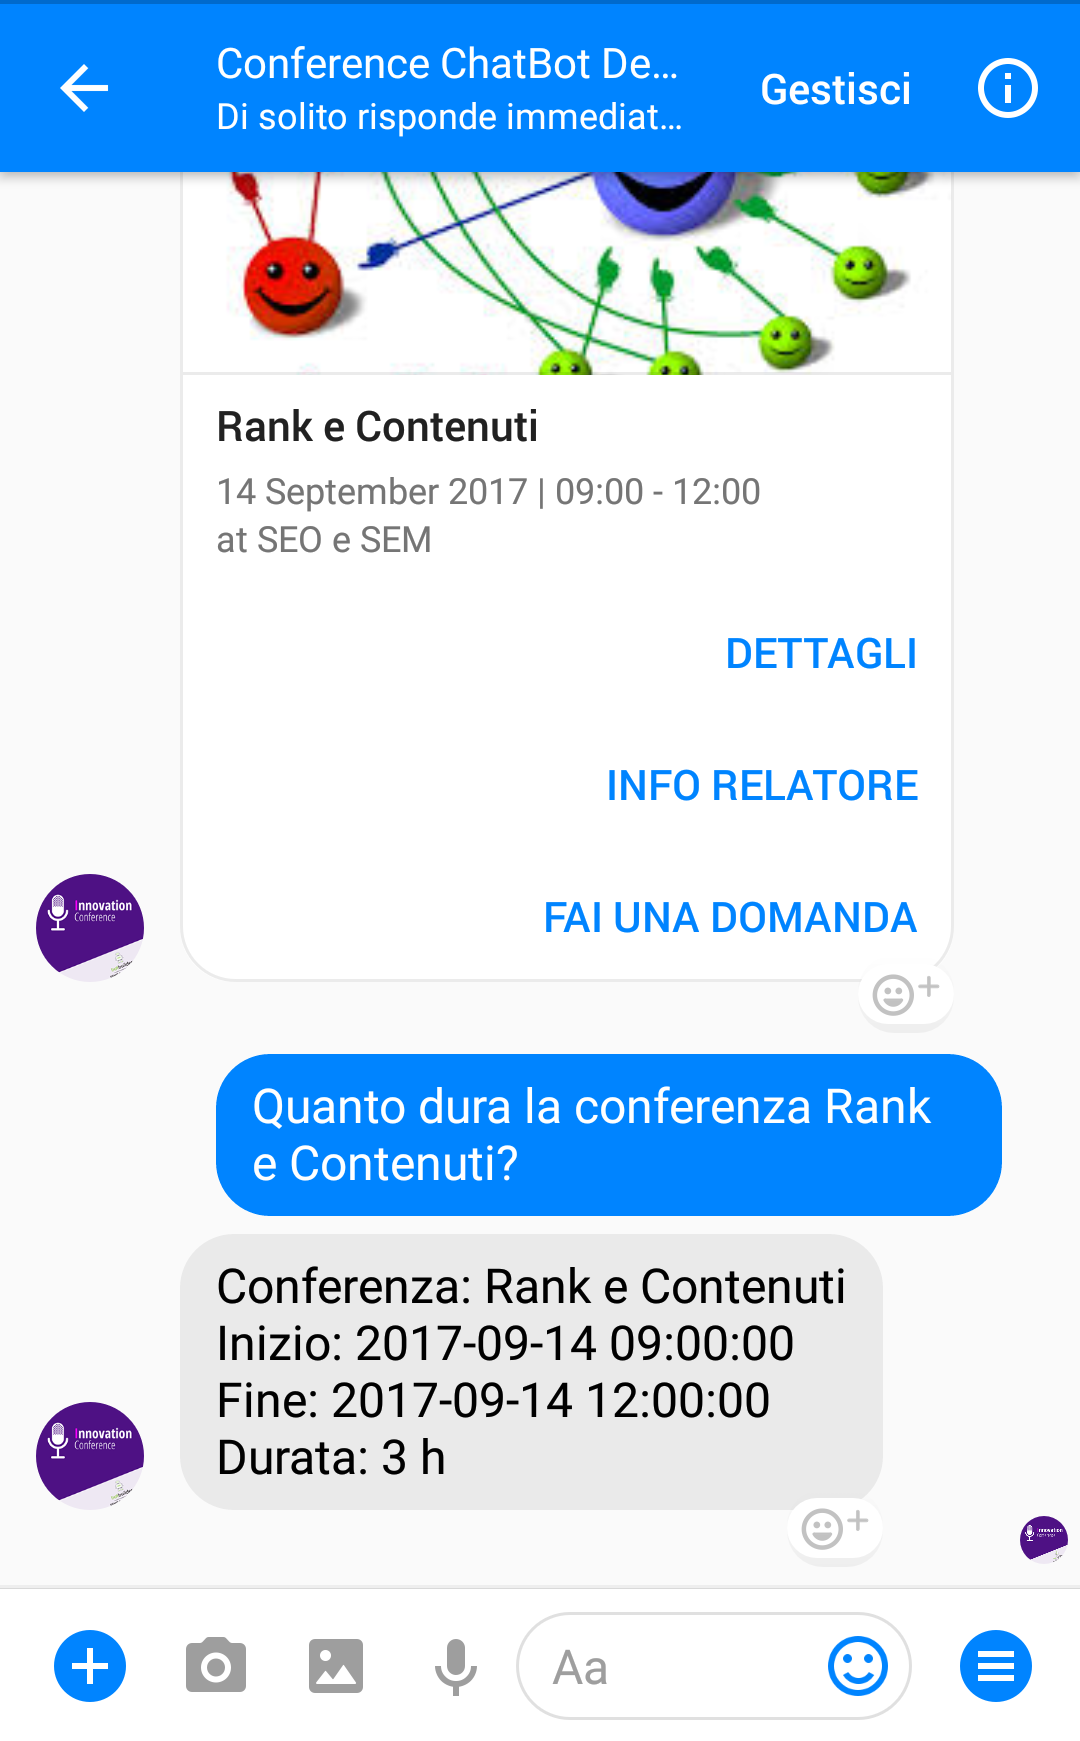
\includegraphics[scale=0.16]{../Immagini/durata.png}
		\caption{Esempio dell'intent durata\_conferenza}
	\end{figure}
\newpage
	\item \textbf{luogo\_conferenza}: permette all'utente di domandare il luogo dove si svolgerà la conferenza. La risposta del \gls{Chatbot} contiene un carosello predefinito da Messenger, con tutte le informazioni sull'aula in questione;
	\begin{figure}[h!]
		\centering
		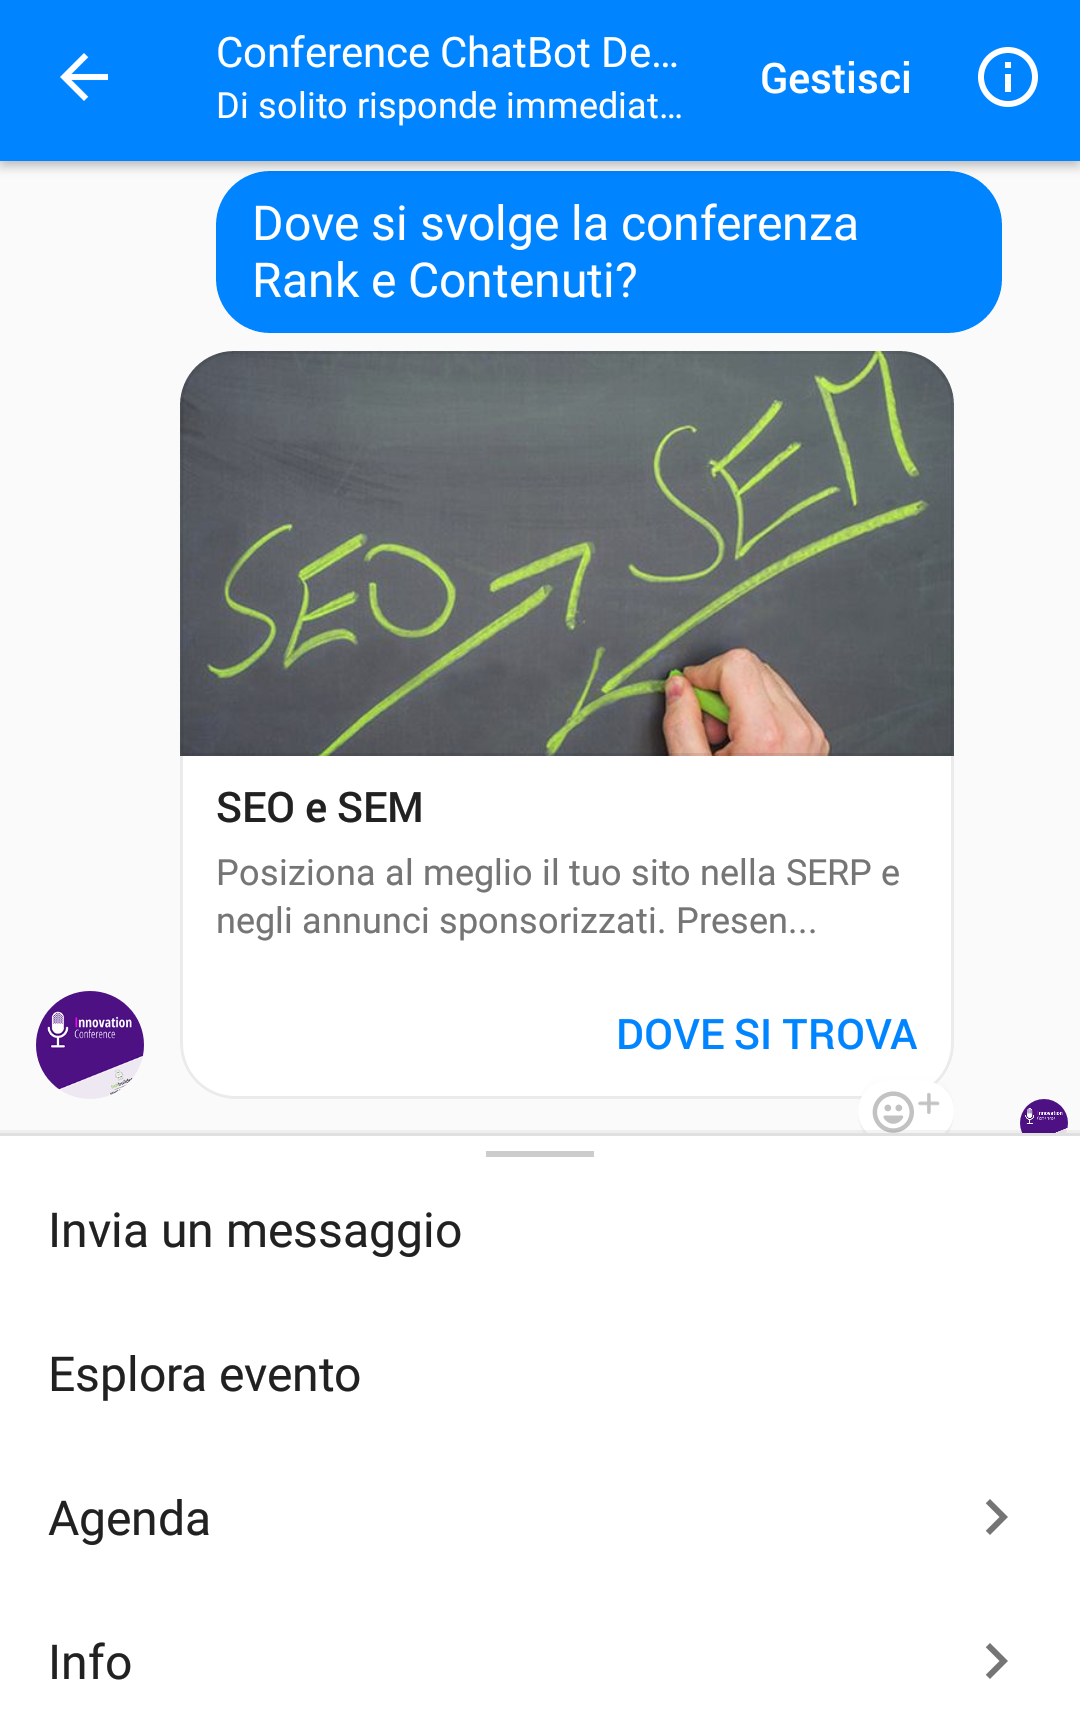
\includegraphics[scale=0.16]{../Immagini/luogo.png}
		\caption{Esempio dell'intent luogo\_conferenza}
	\end{figure}		
	\item \textbf{ora\_conferenza}: permette all'utente di chiedere l'orario di inizio e di fine di una conferenza. La risposta del \gls{Chatbot} contiene un carosello predefinito da Messenger, con tutte le informazioni sulla conferenza;
	\begin{figure}[h!]
		\centering
		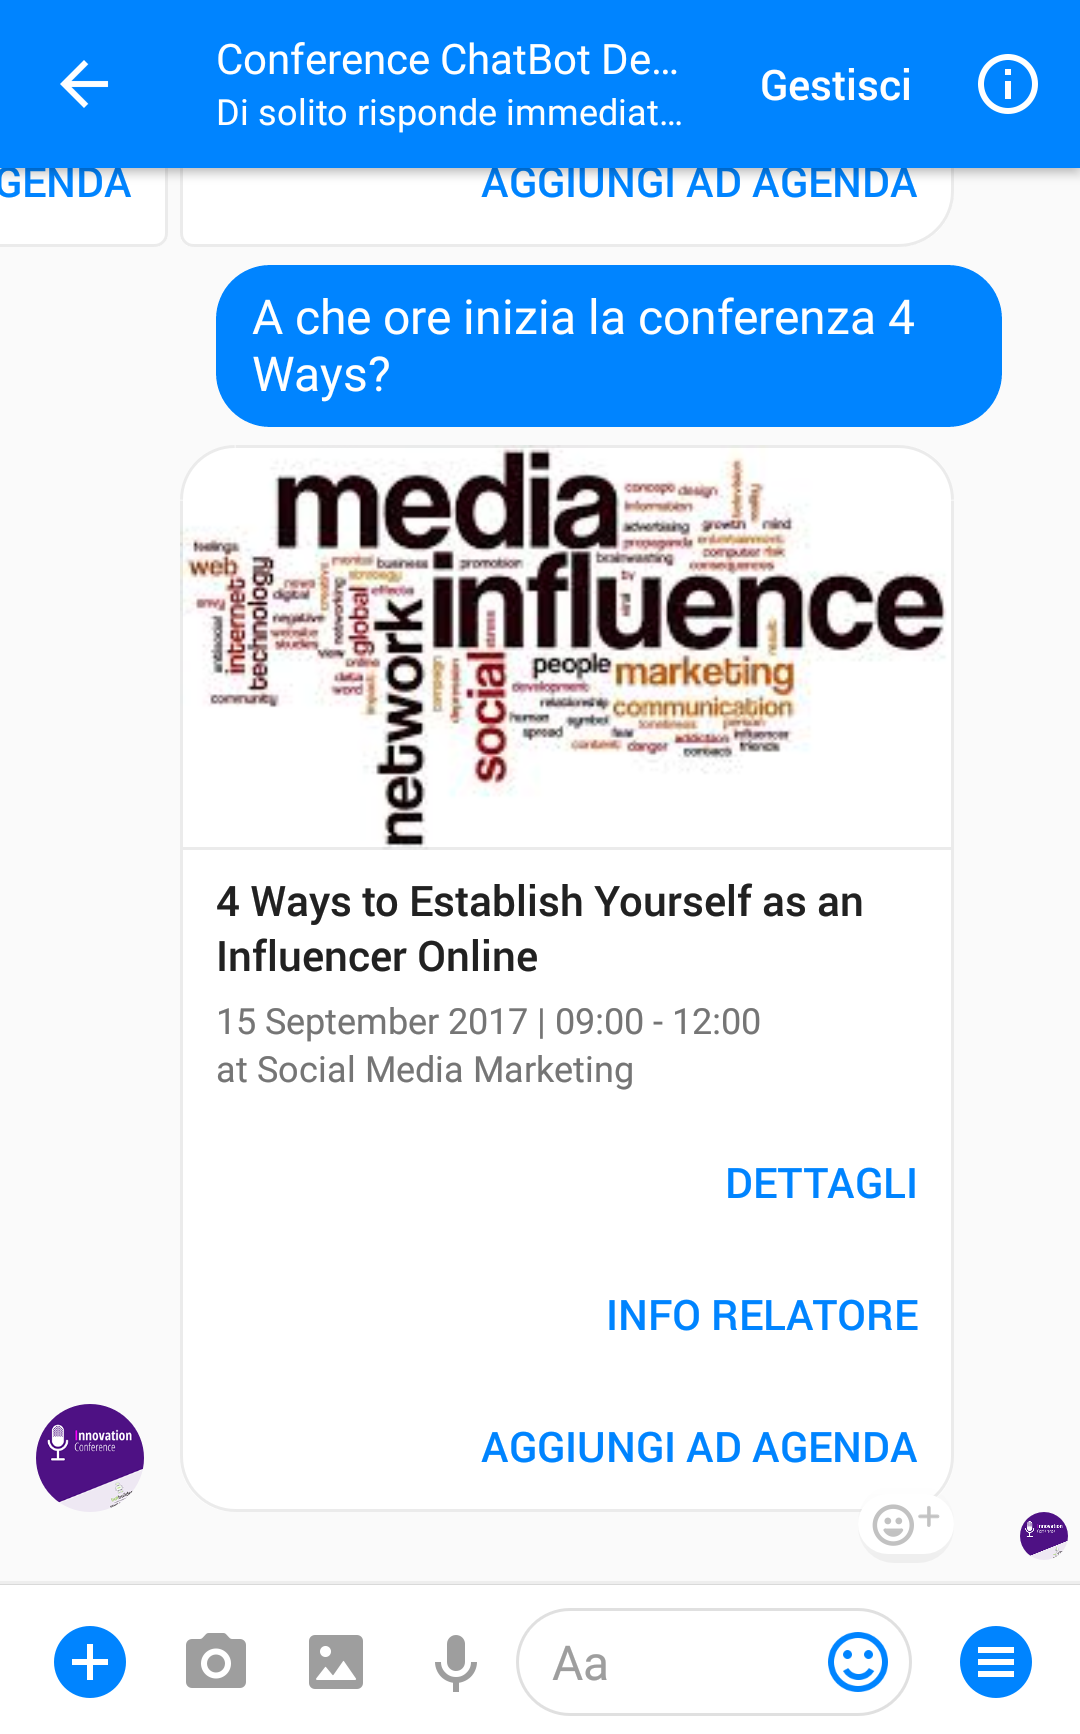
\includegraphics[scale=0.16]{../Immagini/ora_inizio.png}
		\caption{Esempio dell'intent ora\_conferenza}
	\end{figure}	
\newpage	
	\item \textbf{indicazioni\_stanza}: permette all'utente di domandare le indicazioni per trovare una determinata aula. La risposta del \gls{Chatbot} contiene le indicazioni presenti nel database, con una piccola mappa illustrativa;
	\begin{figure}[h!]
		\centering
		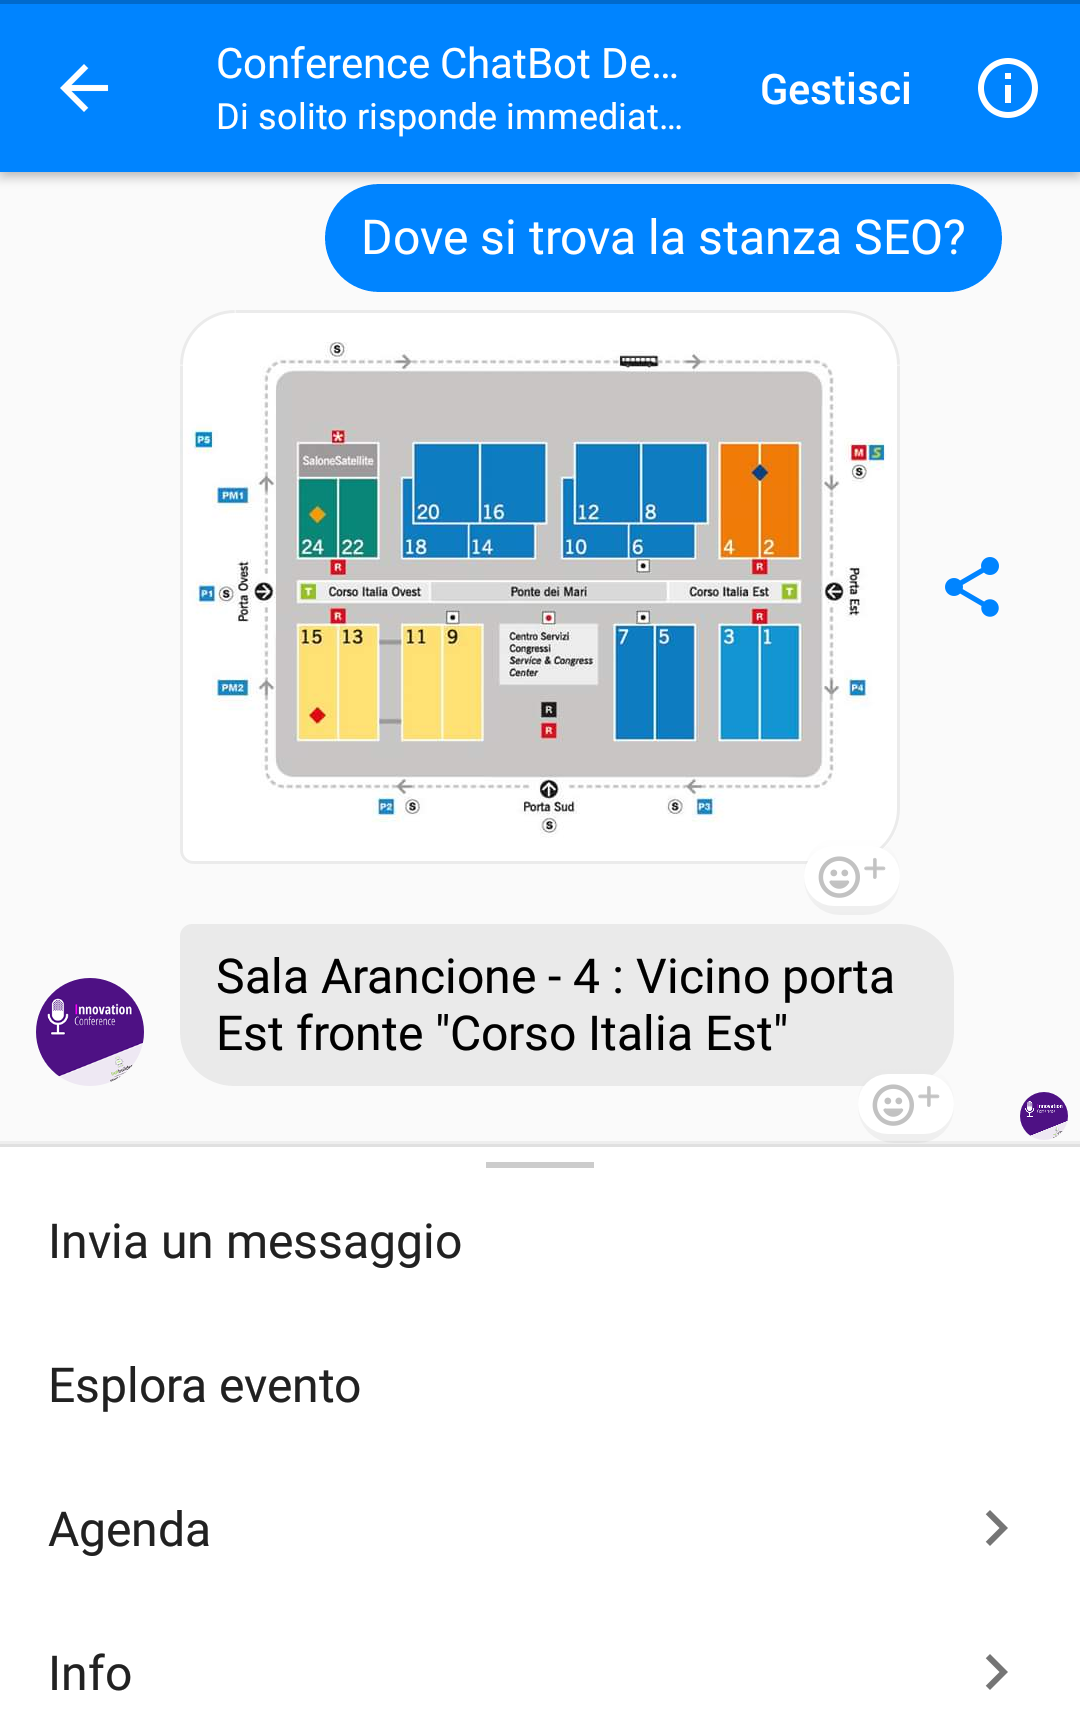
\includegraphics[scale=0.16]{../Immagini/indicazioni.png}
		\caption{Esempio dell'intent indicazioni\_stanza}
	\end{figure}			
	\item \textbf{programma\_giornata}: permette all'utente di domandare il programma dell'evento di un determinato giorno. La risposta del \gls{Chatbot} contiene un carosello per ogni conferenza in programma quel giorno;
	\begin{figure}[h!]
		\centering
		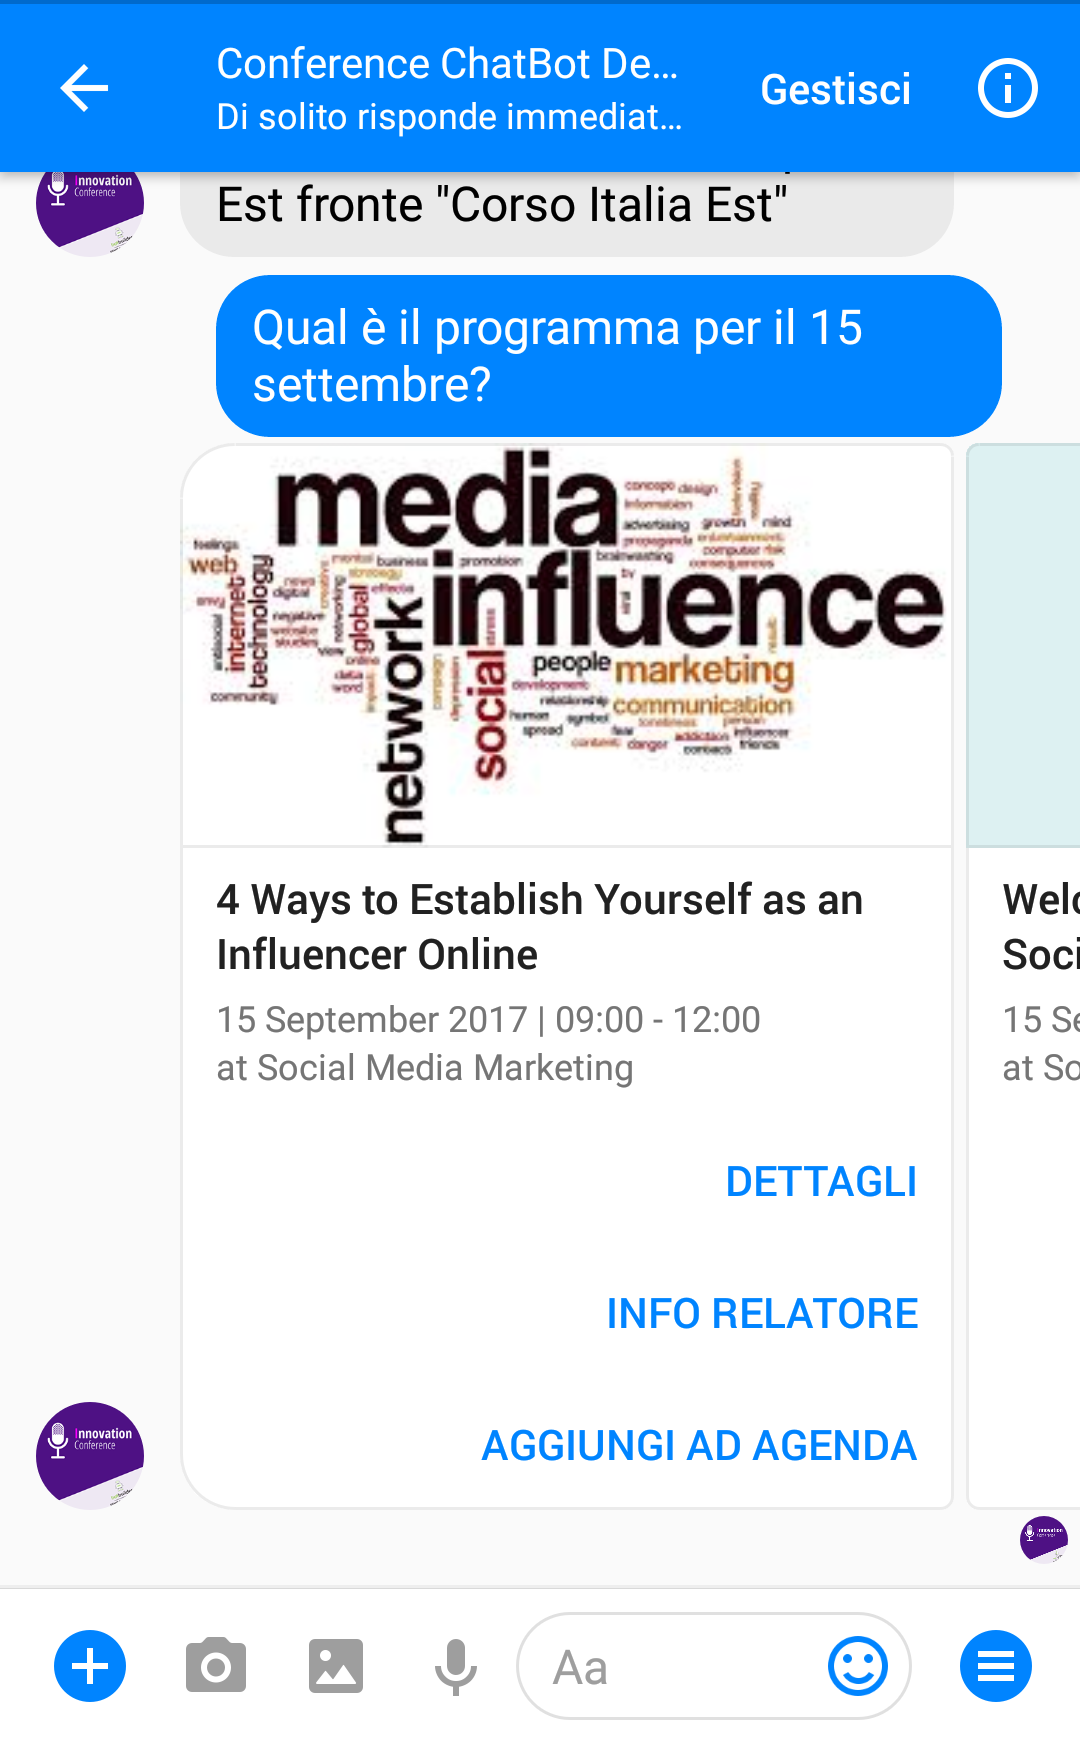
\includegraphics[scale=0.16]{../Immagini/programma_data.png}
		\caption{Esempio dell'intent programma\_giornata}
	\end{figure}			
	\item \textbf{programma\_no\_data}: permette all'utente di domandare quale conferenza si sta svolgendo in quel momento in una determinata stanza. La risposta del \gls{Chatbot} contiene un carosello con la conferenza in programma;
	\begin{figure}[h!]
		\centering
		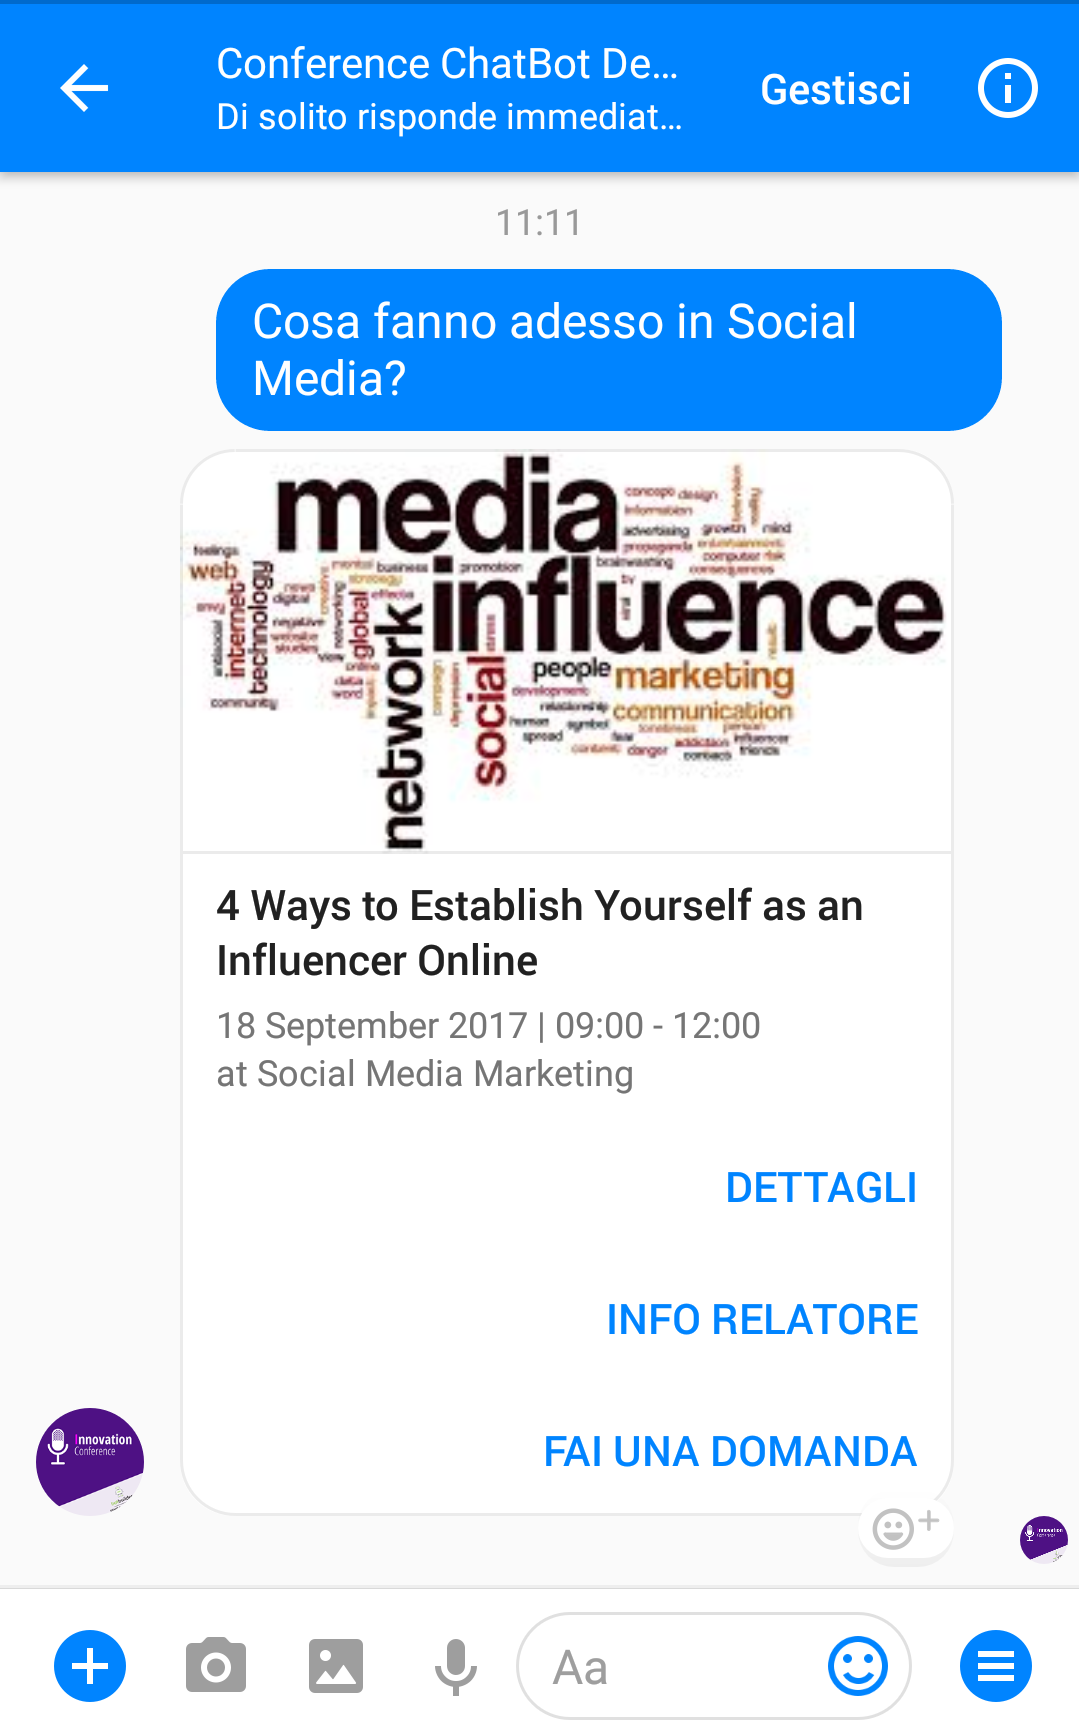
\includegraphics[scale=0.16]{../Immagini/adesso.png}
		\caption{Esempio dell'intent programma\_no\_data}
	\end{figure}			
	\item \textbf{data\_ora\_stanza\_conferenza}: permette all'utente di domandare la conferenza in programma specificando data, ora e aula. La risposta del \gls{Chatbot} contiene un carosello con la conferenza in programma, se presente;
	\begin{figure}[h!]
		\centering
		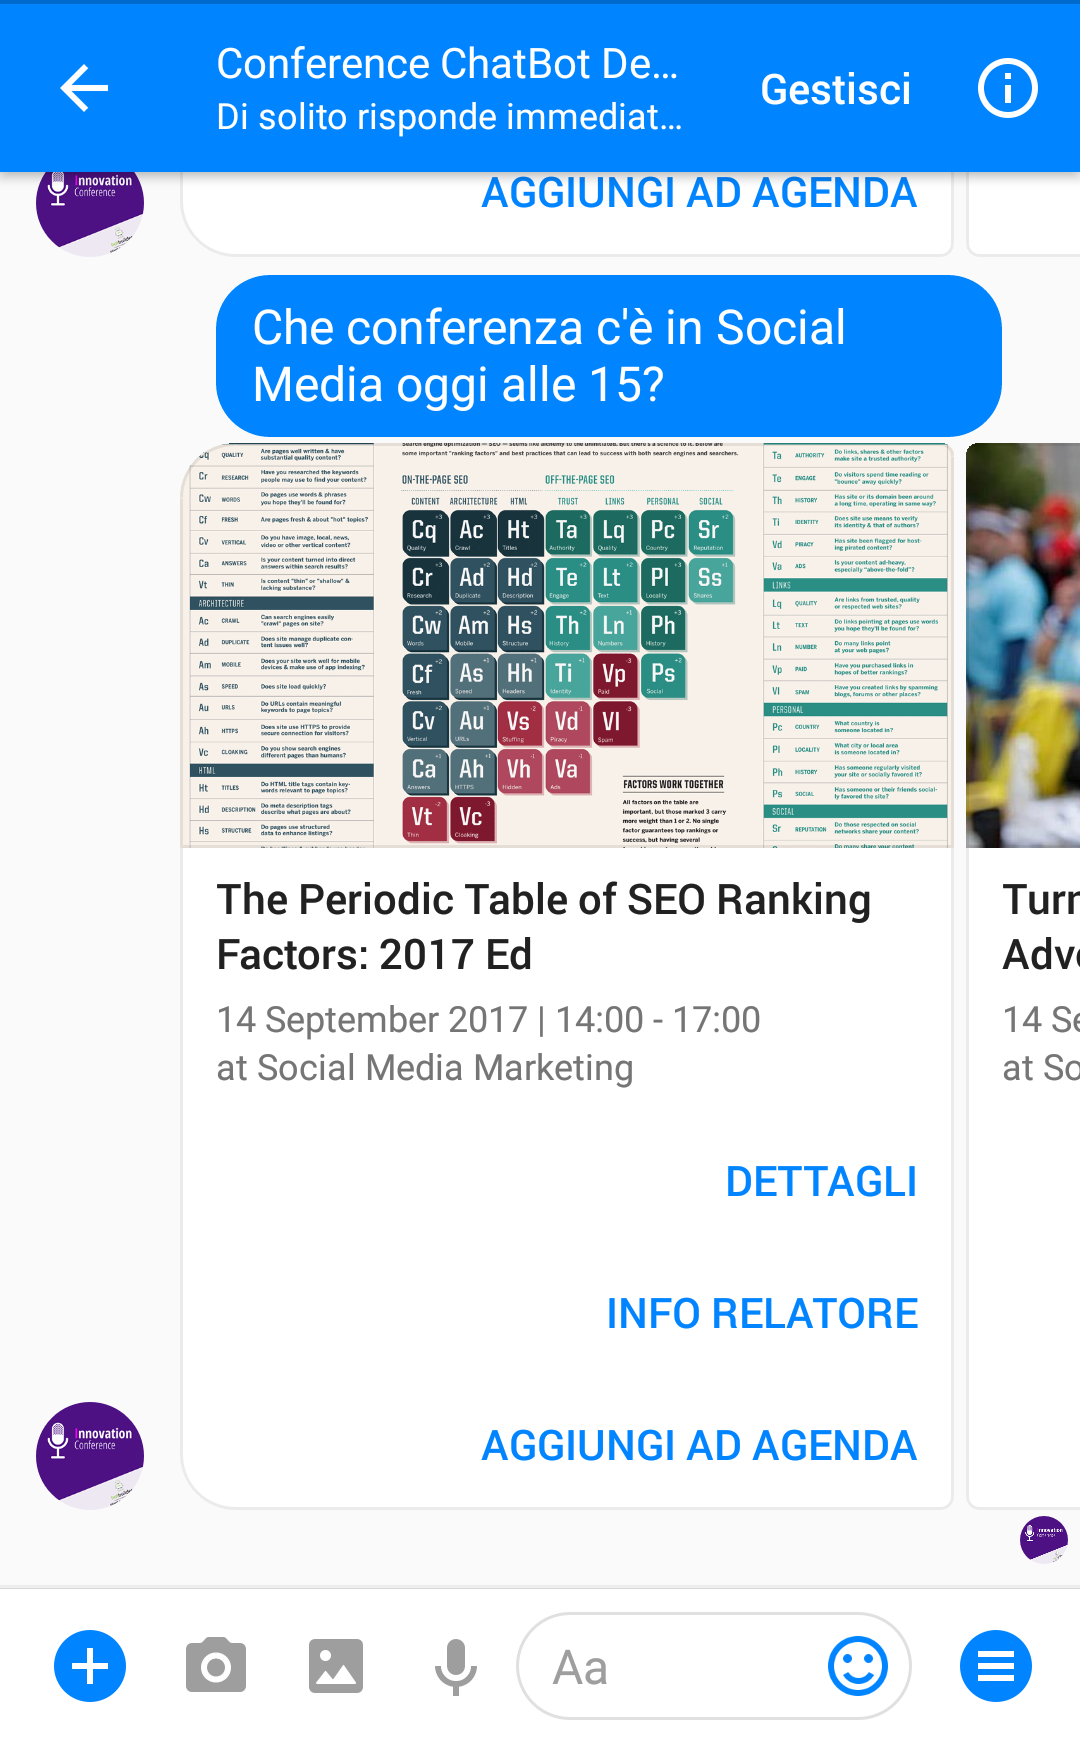
\includegraphics[scale=0.16]{../Immagini/stanza_data_ora.png}
		\caption{Esempio dell'intent data\_ora\_stanza\_conferenza}
	\end{figure}			
	\item \textbf{data\_stanza\_conferenza}: permette all'utente di domandare la conferenza in programma specificando data e aula. La risposta del \gls{Chatbot} contiene un carosello con la conferenza in programma, se presente;
	\begin{figure}[h!]
		\centering
		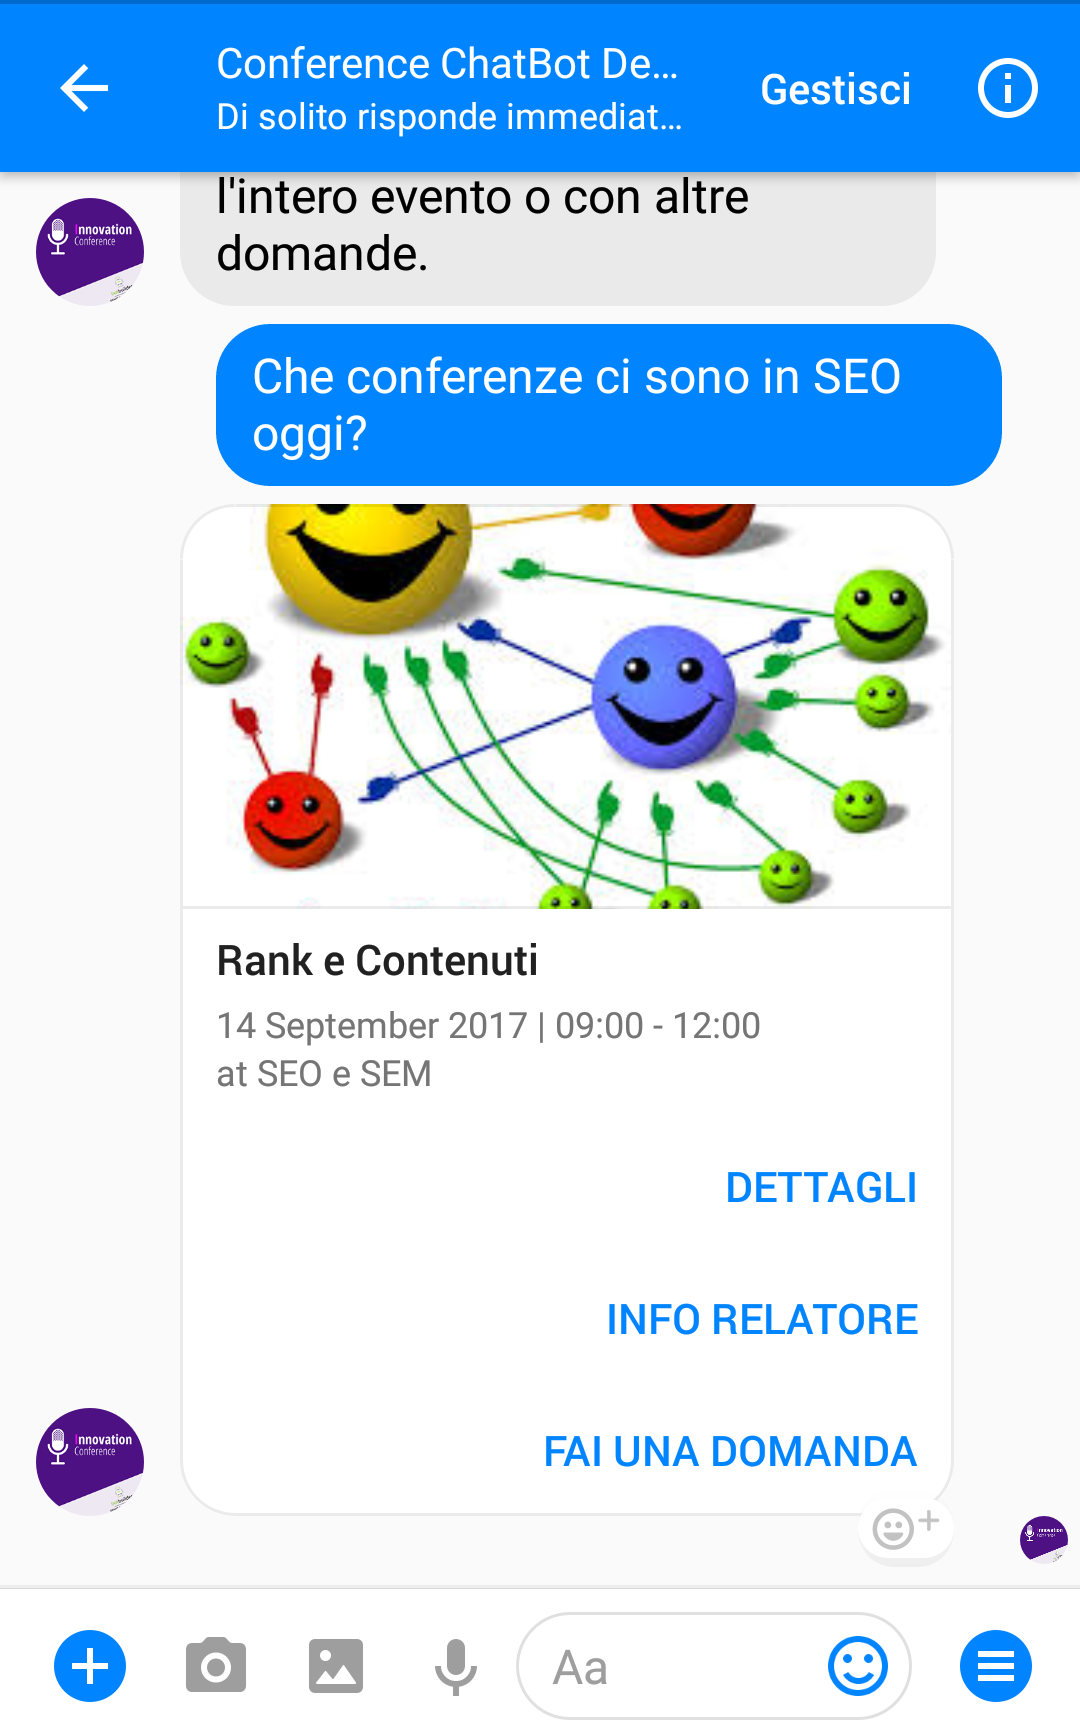
\includegraphics[scale=0.16]{../Immagini/stanza_data.png}
		\caption{Esempio dell'intent data\_stanza\_conferenza}
	\end{figure}			
	\item \textbf{ora\_stanza\_conferenza}: permette all'utente di domandare la conferenza in programma specificando ora e aula. La risposta del \gls{Chatbot} contiene un carosello con la conferenza in programma, se presente;
	\begin{figure}[h!]
		\centering
		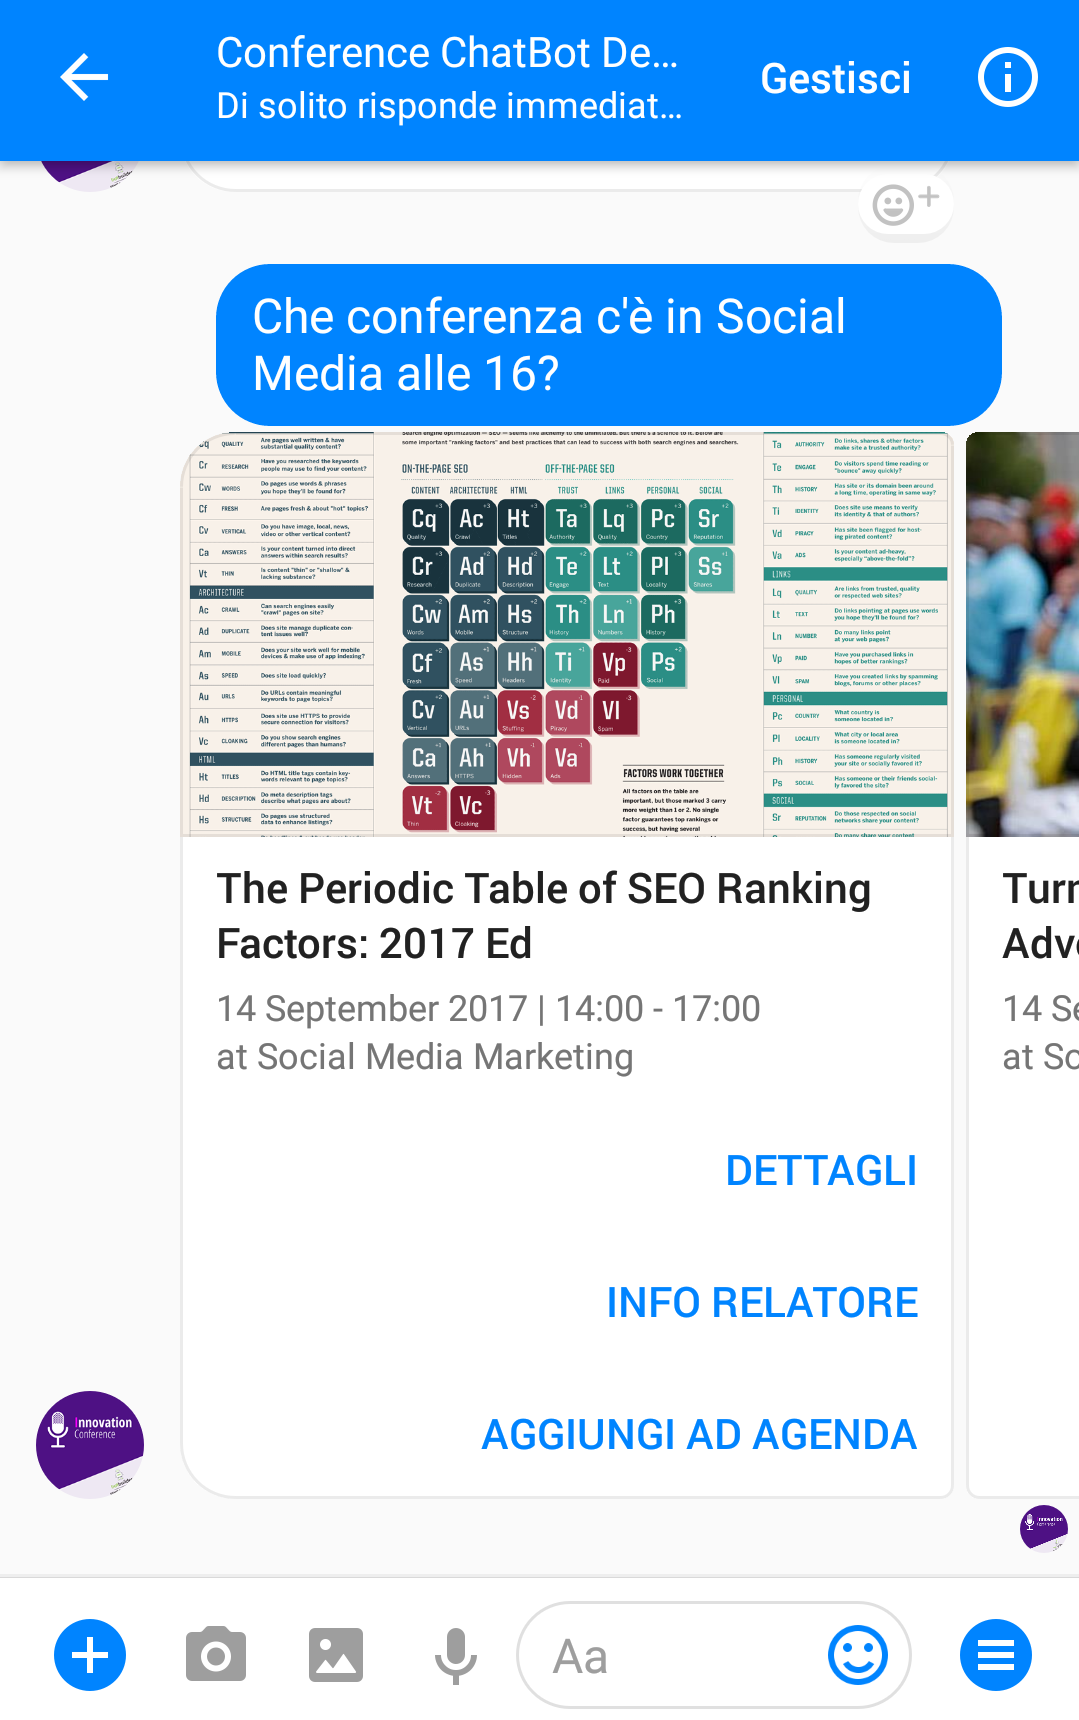
\includegraphics[scale=0.16]{../Immagini/stanza_ora.png}
		\caption{Esempio dell'intent ora\_stanza\_conferenza}
	\end{figure}		
	\item \textbf{visualizza\_agenda}: permette all'utente di visualizzare la propria agenda (cioè le conferenze che ha aggiunto precedentemente). La risposta contiene tutte le conferenze aggiunte all'agenda;
	\begin{figure}[h!]
		\centering
		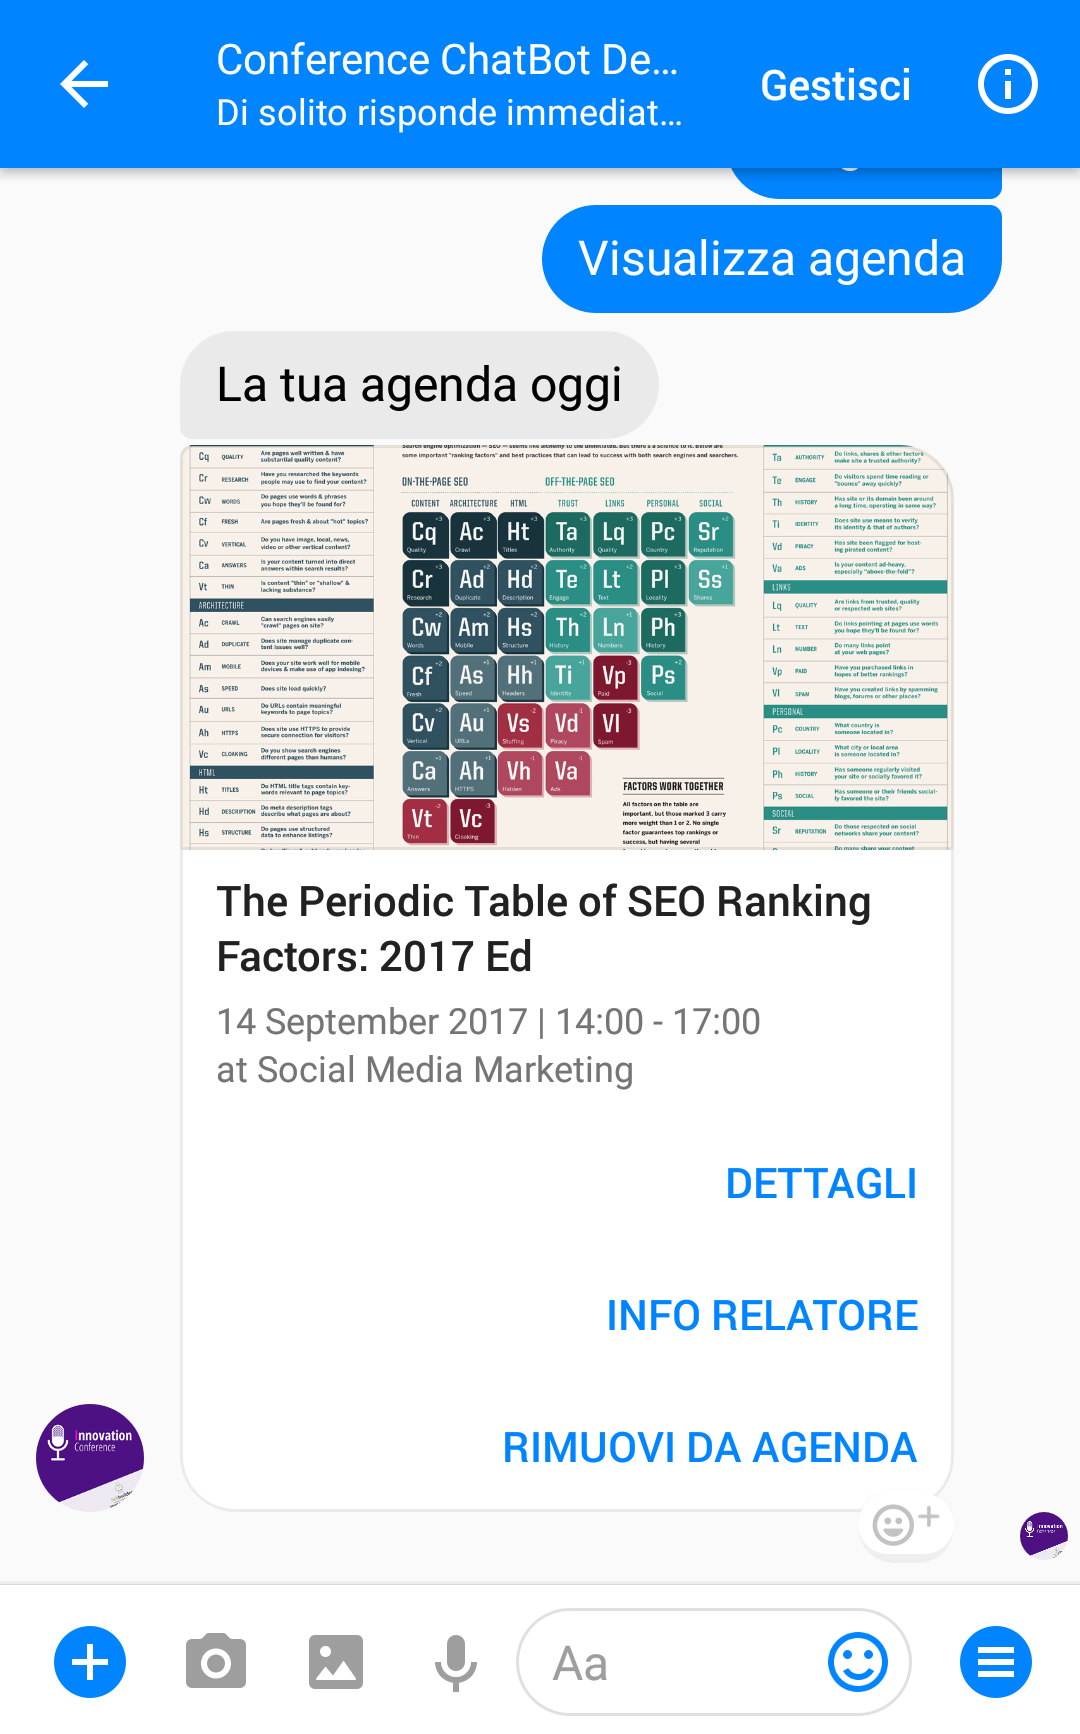
\includegraphics[scale=0.16]{../Immagini/agenda.png}
		\caption{Esempio dell'intent visualizza\_agenda}
	\end{figure}			
	\item \textbf{richiesta\_aiuto}: permette all'utente di ottenere delle informazioni per l'utilizzo del \gls{Chatbot}. La risposta contiene una breve spiegazione e delle domande che possono essere rivolte al bot.
	\begin{figure}[h!]
		\centering
		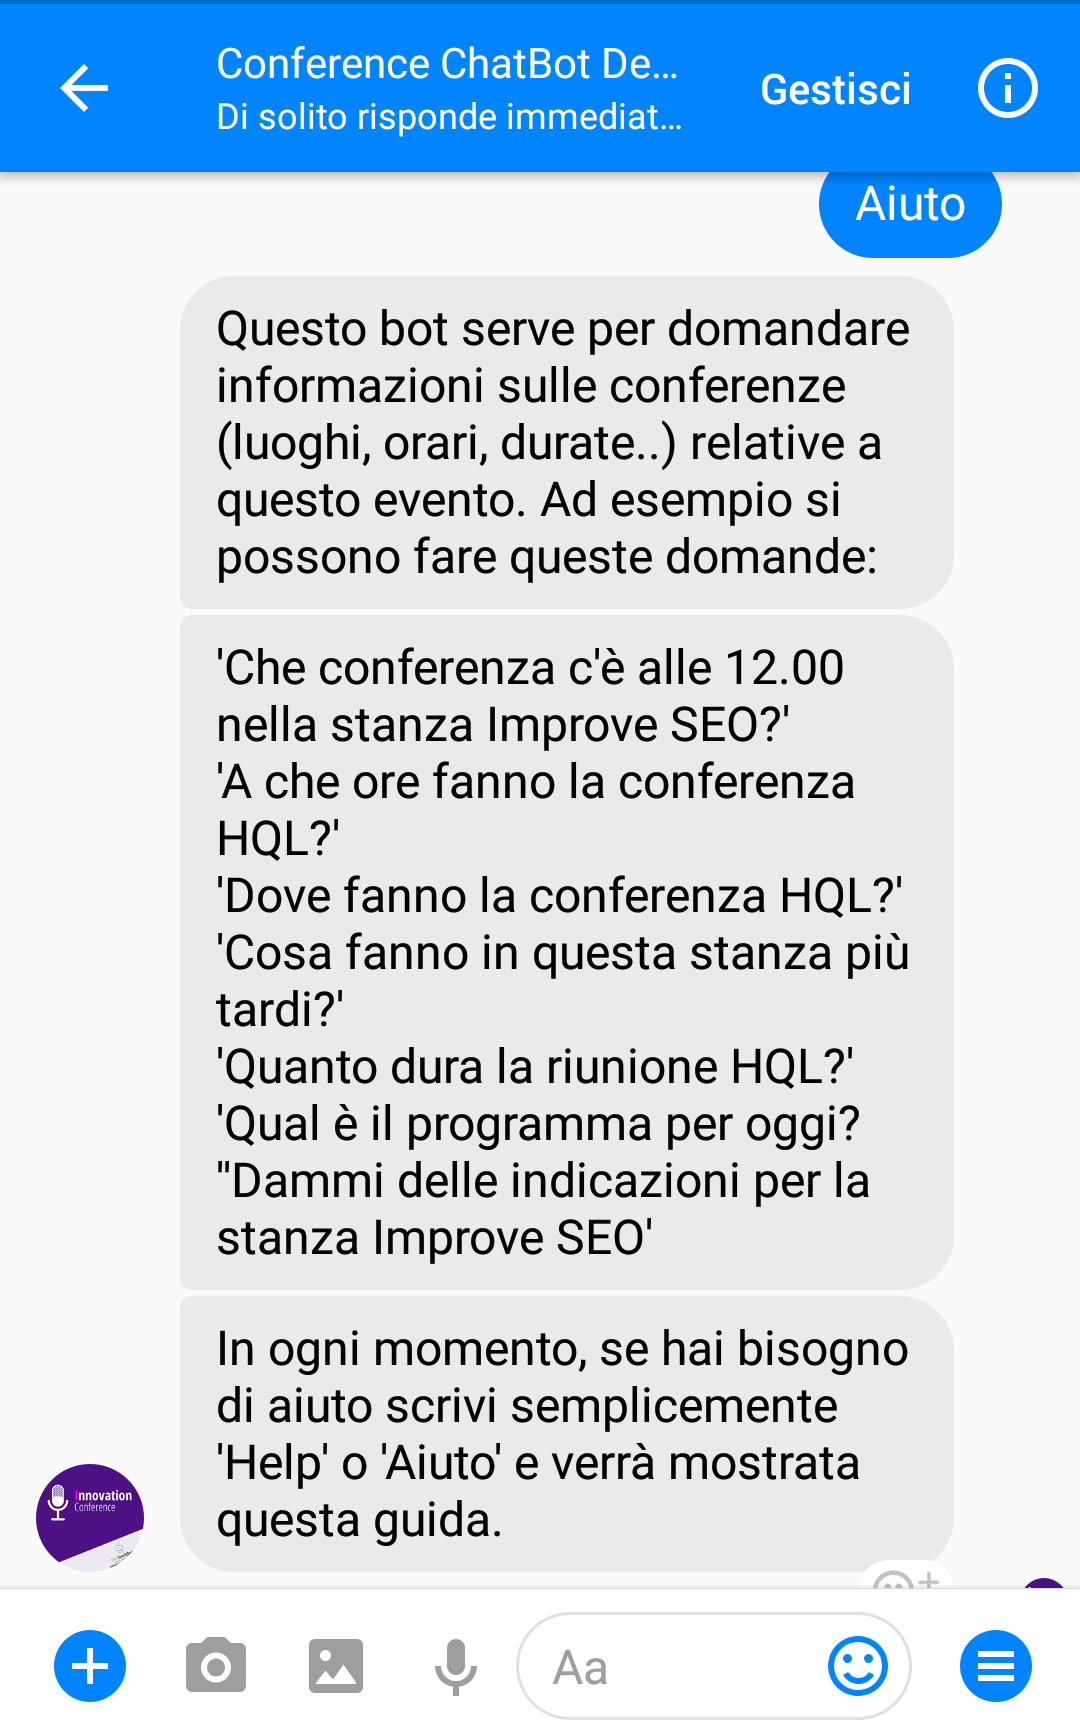
\includegraphics[scale=0.16]{../Immagini/aiuto.png}
		\caption{Esempio dell'intent richiesta\_aiuto}
	\end{figure}	
\end{itemize}
\newpage
\subsubsection{Entity}
Nella progettazione di questo \emph{agent} ho creato queste nuove \emph{entities}:
\begin{itemize}
	\item \textbf{conference}: viene utilizzata per gestire i sinonimi della parola "conferenza". In questo modo scrivere assemblea, meeting ha lo stesso risultato di conferenza;
	\item \textbf{stanza}: viene utilizzata per gestire i sinonimi della parola "stanza". In questo modo l'utente può scrivere aula, sala, padiglione con lo stesso risultato di stanza;
	\item \textbf{my\_time}: questa \emph{entity} è formata da \emph{@sys.time}, ossia una \emph{system entity} fornita da api.ai per estrarre un orario dall'input dell'utente, e una serie di espressioni per indicare il momento attuale in cui l'utente fa la domanda (adesso, in questo momento, ora). In questo modo se l'utente scrive \emph{"Cosa fanno in aula X adesso?"}, nel \gls{JSON} ritornato da api.ai ci sarà un parametro di tipo \emph{my\_time} con valore "adesso", che potrà essere gestito nella \emph{business logic}.
\end{itemize}

\begin{figure}[h!]
	\centering
	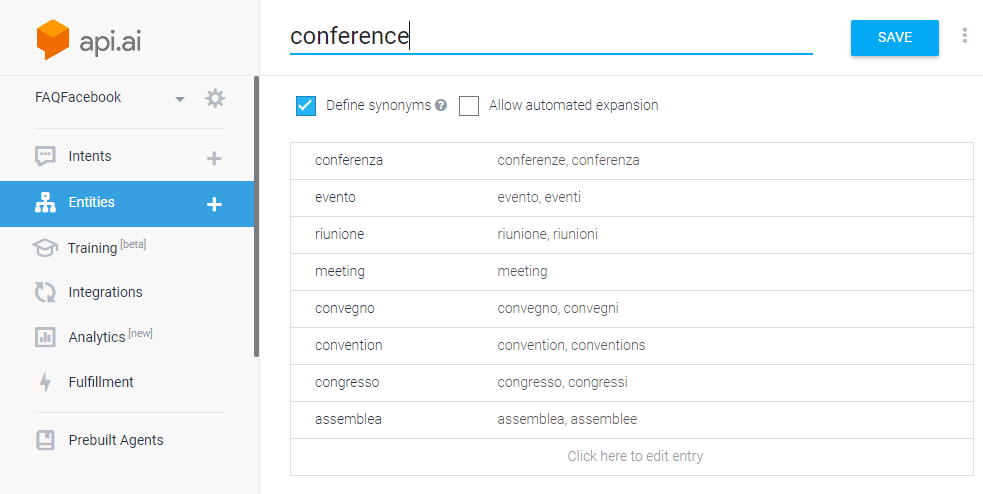
\includegraphics[scale=0.5]{../Immagini/conference.png}
	\caption{Entity conference definita nell'agent}
\end{figure}

\subsection{Dati ARPA Veneto}
Il \gls{Chatbot} dedicato al meteo è stato realizzato grazie agli \emph{open data} messi a disposizione dall'Agenzia Regionale per la Prevenzione e Protezione Ambientale del Veneto(ARPAV). Ogni giorno, nel sito ufficiale\footcite{arpav}, vengono emessi tre bollettini:
\begin{itemize}
	\item \textbf{alle 9:00}: che rappresenta un aggiornamento del bollettino del giorno precedente;
	\item \textbf{alle 13:00}: il nuovo bollettino;
	\item \textbf{alle 16:00}: un aggiornamento del bollettino emesso alle 13.
\end{itemize} 

Il file \gls{Extensible Markup Language} che è possibile scaricare, contiene queste informazioni:
\begin{itemize}
	\item le previsioni dei cinque giorni successivi per le 18 zone in cui è stata divisa la regione del Veneto;
	\item una descrizione dell'evoluzione generale dei cinque giorni successivi, per tre macro zone: la regione intera, la zona delle Dolomiti e la pianura veneta.
\end{itemize}

Ad ogni nuova emissione del bollettino, i nuovi dati vengono inseriti nel database aziendale, in modo da comunicare agli utenti solamente le notizie più aggiornate.

\subsection{Meteo Veneto Bot}
\subsubsection{Intent}
Gli intents che ho deciso di creare per soddisfare tutti i requisiti sono i seguenti:
\begin{itemize}
	\item \textbf{richiesta\_meteo}: permette all'utente di chiedere le previsioni del meteo specificando una giornata o un periodo di tempo (es. weekend) e il comune di interesse (se non viene specificato, si considera il comune da lui selezionato all'inizio dell'interazione con il \gls{Chatbot}). La risposta contiene un carosello con il meteo richiesto.
	\begin{figure}[h]
		\centering
		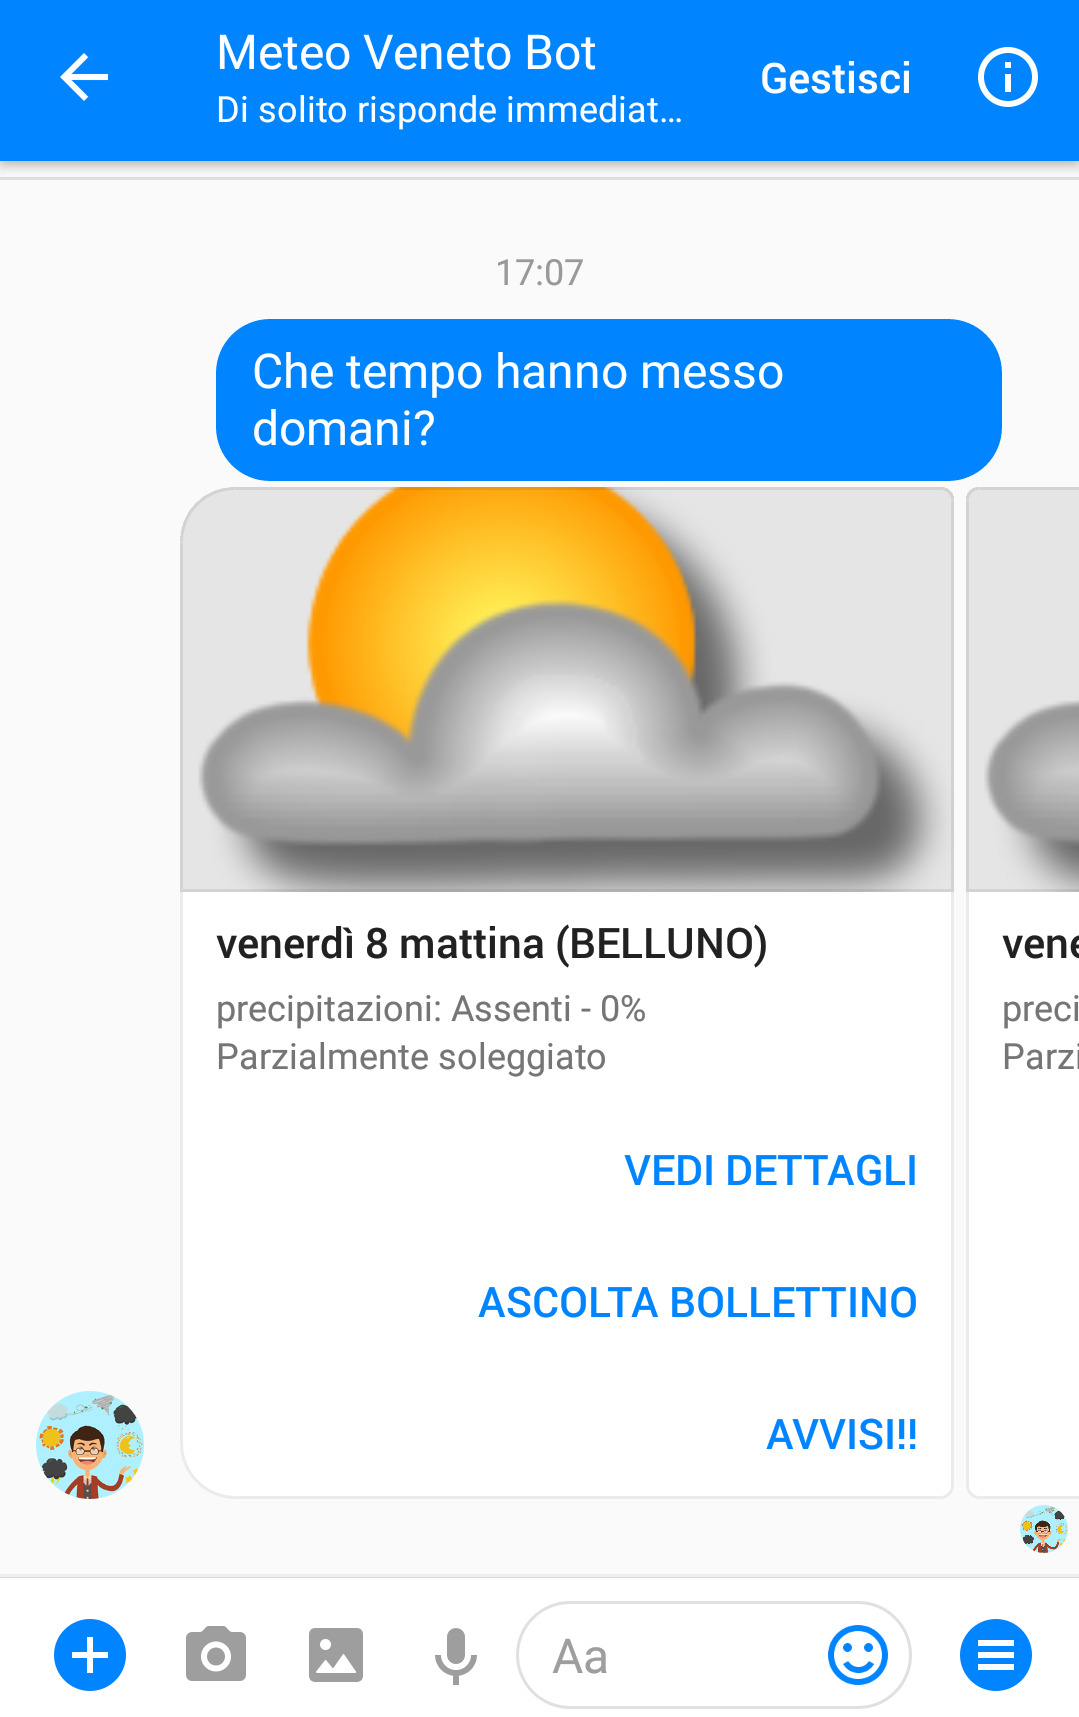
\includegraphics[scale=0.15]{../Immagini/richiesta_meteo.png}
		\caption{Esempio dell'intent richiesta\_meteo}
	\end{figure}	
\newpage
	\item \textbf{richiesta\_sole}: permette all'utente di chiedere se è previsto il sole in una specifica giornata o un periodo di tempo (es. weekend), in un determinato comune. La risposta è formata da due messaggi: il primo mostra le giornate dove è previsto il sole, tra quelle richieste dall'utente, il secondo contiene i caroselli delle previsioni.
	\begin{figure}[!h]
		\centering
		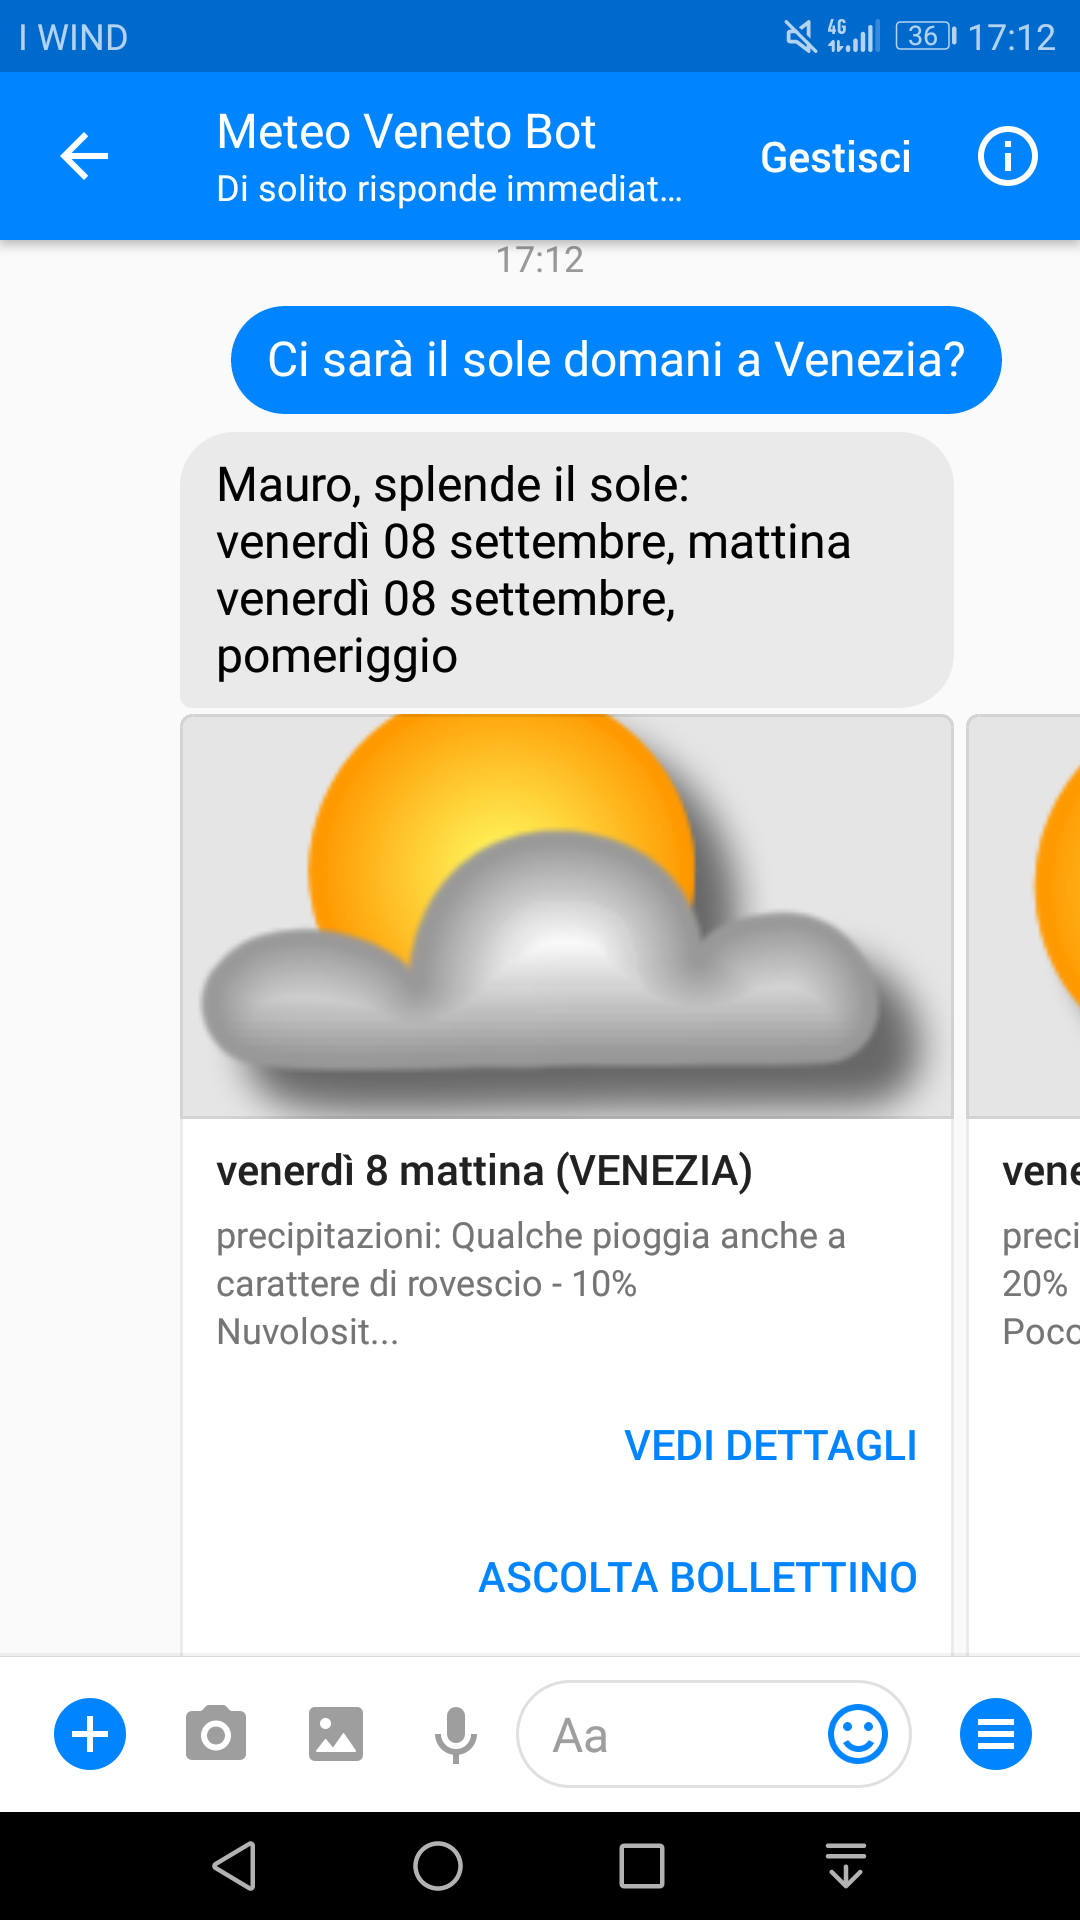
\includegraphics[scale=0.15]{../Immagini/richiesta_sole.png}
		\caption{Esempio dell'intent richiesta\_sole}
	\end{figure}	
	\item \textbf{richiesta\_pioggia}: permette all'utente di chiedere se è prevista pioggia in una specifica giornata o un periodo di tempo (es. weekend), in un determinato comune. La risposta è formata da due messaggi: il primo mostra le giornate dove è prevista pioggia, tra quelle richieste dall'utente, il secondo contiene i caroselli delle previsioni.
	\begin{figure}[!h]
		\centering
		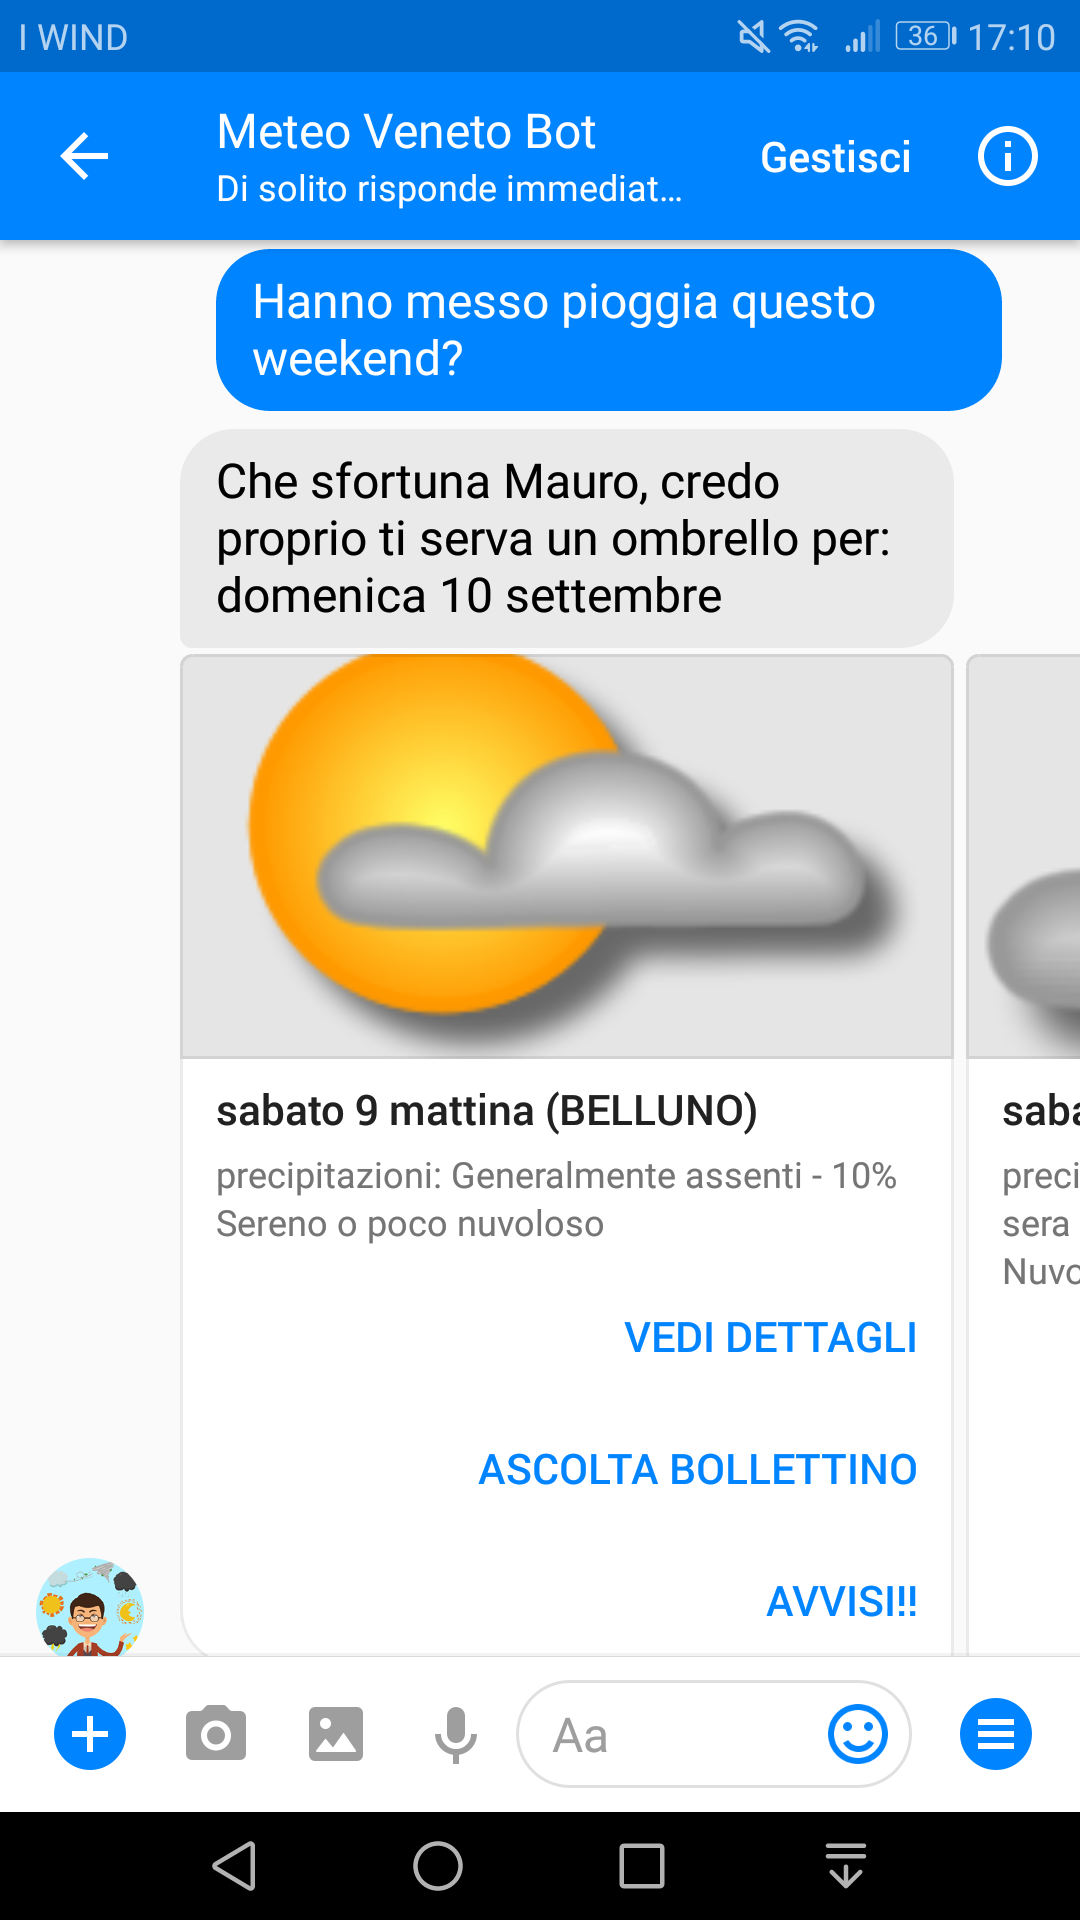
\includegraphics[scale=0.15]{../Immagini/richiesta_pioggia.png}% "%" necessario
		\qquad\qquad
		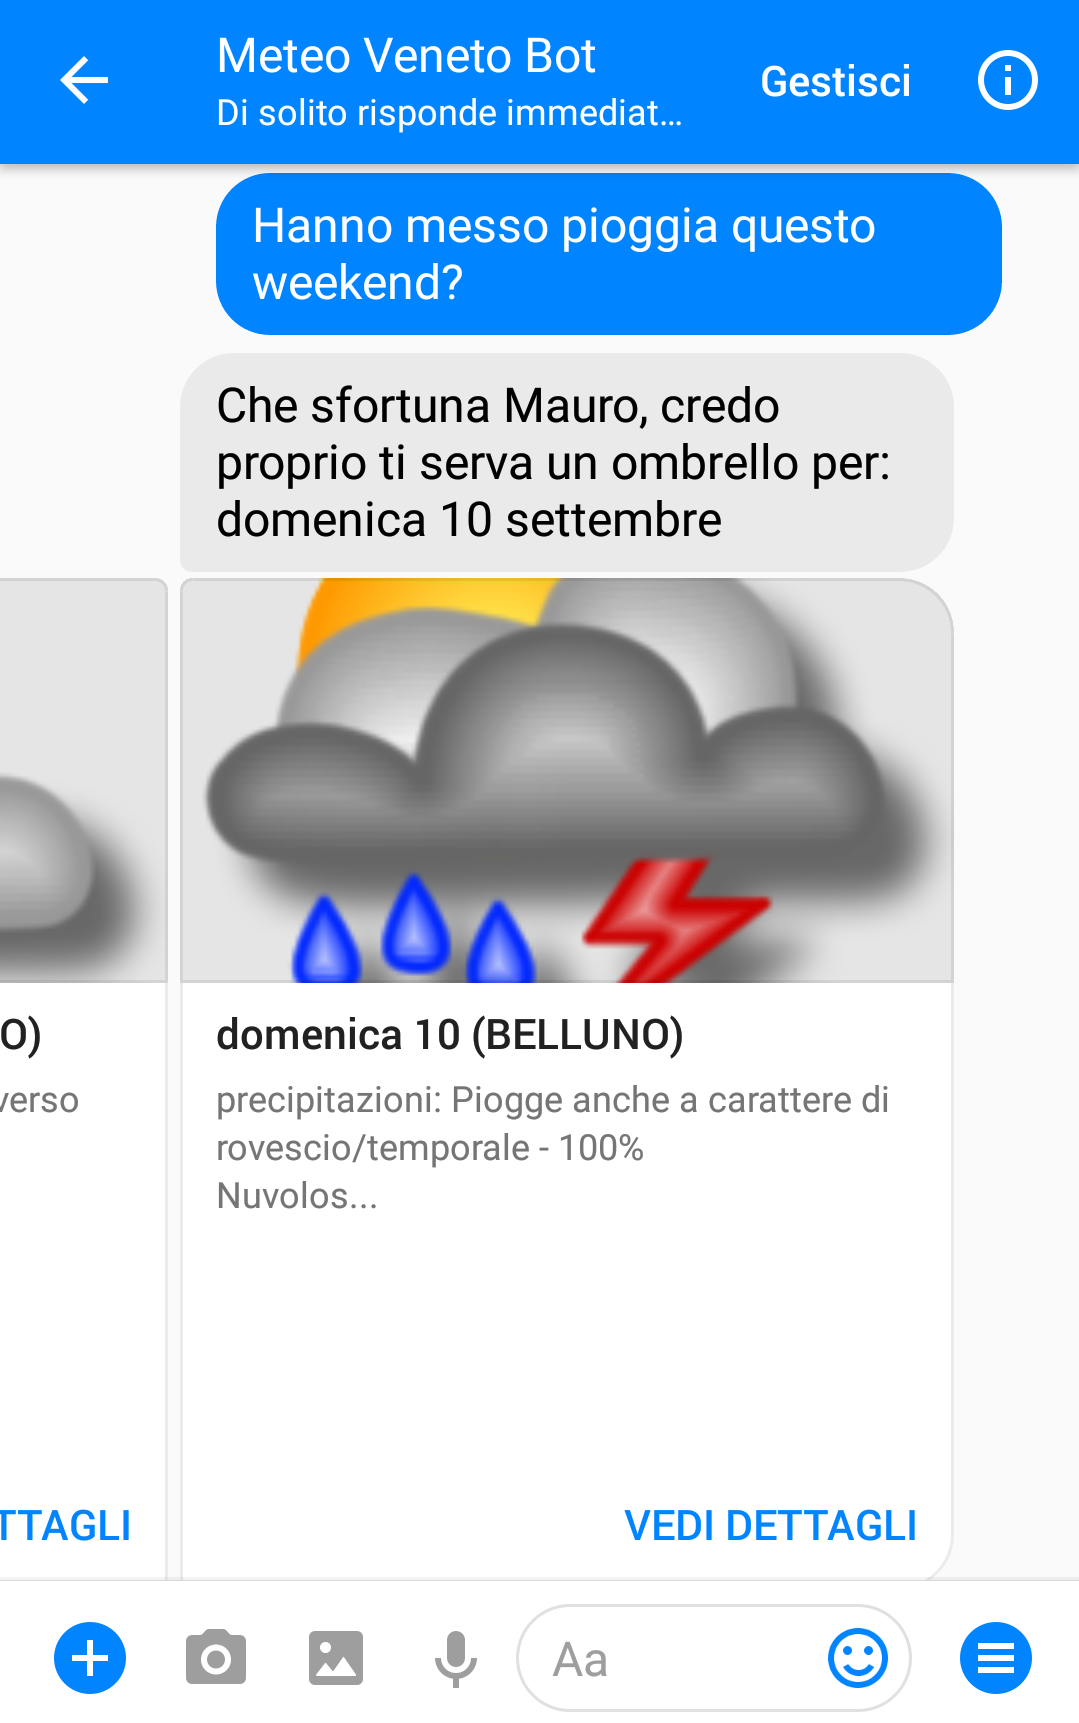
\includegraphics[scale=0.15]{../Immagini/richiesta_pioggia2.png}
		\caption{Esempio dell'intent richiesta\_pioggia}
	\end{figure}
	\item \textbf{richiesta\_nebbia}: permette all'utente di chiedere se è prevista nebbia in una specifica giornata o un periodo di tempo (es. weekend), in un determinato comune. La risposta è formata da due messaggi: il primo mostra le giornate dove è prevista nebbia, tra quelle richieste dall'utente, il secondo contiene i caroselli delle previsioni.
	\begin{figure}[!h]
		\centering
		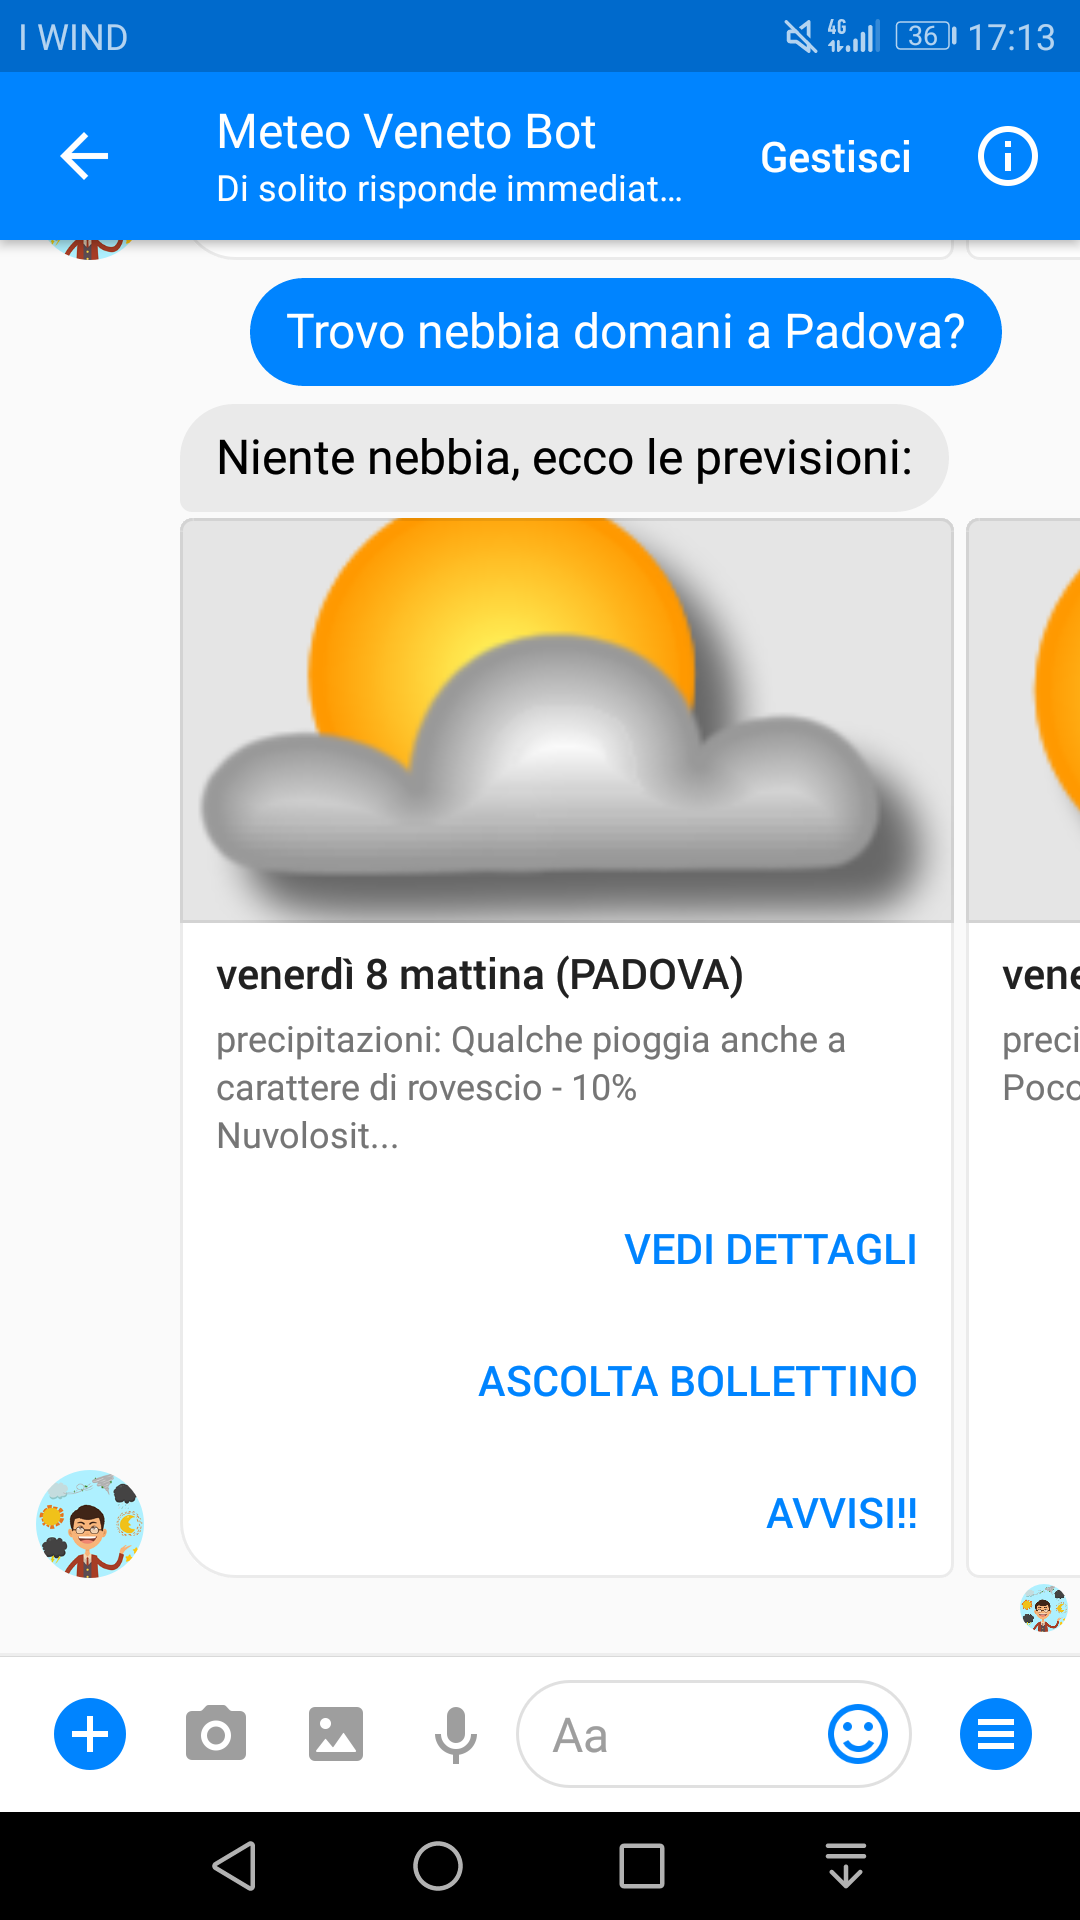
\includegraphics[scale=0.15]{../Immagini/richiesta_nebbia.png}
		\caption{Esempio dell'intent richiesta\_nebbia}
	\end{figure}
	\item \textbf{richiesta\_neve}: permette all'utente di chiedere se è prevista neve in una specifica giornata o un periodo di tempo (es. weekend), in un determinato comune. La risposta è formata da due messaggi: il primo mostra le giornate dove è prevista neve, tra quelle richieste dall'utente, il secondo contiene i caroselli delle previsioni.
	\begin{figure}[!h]
		\centering
		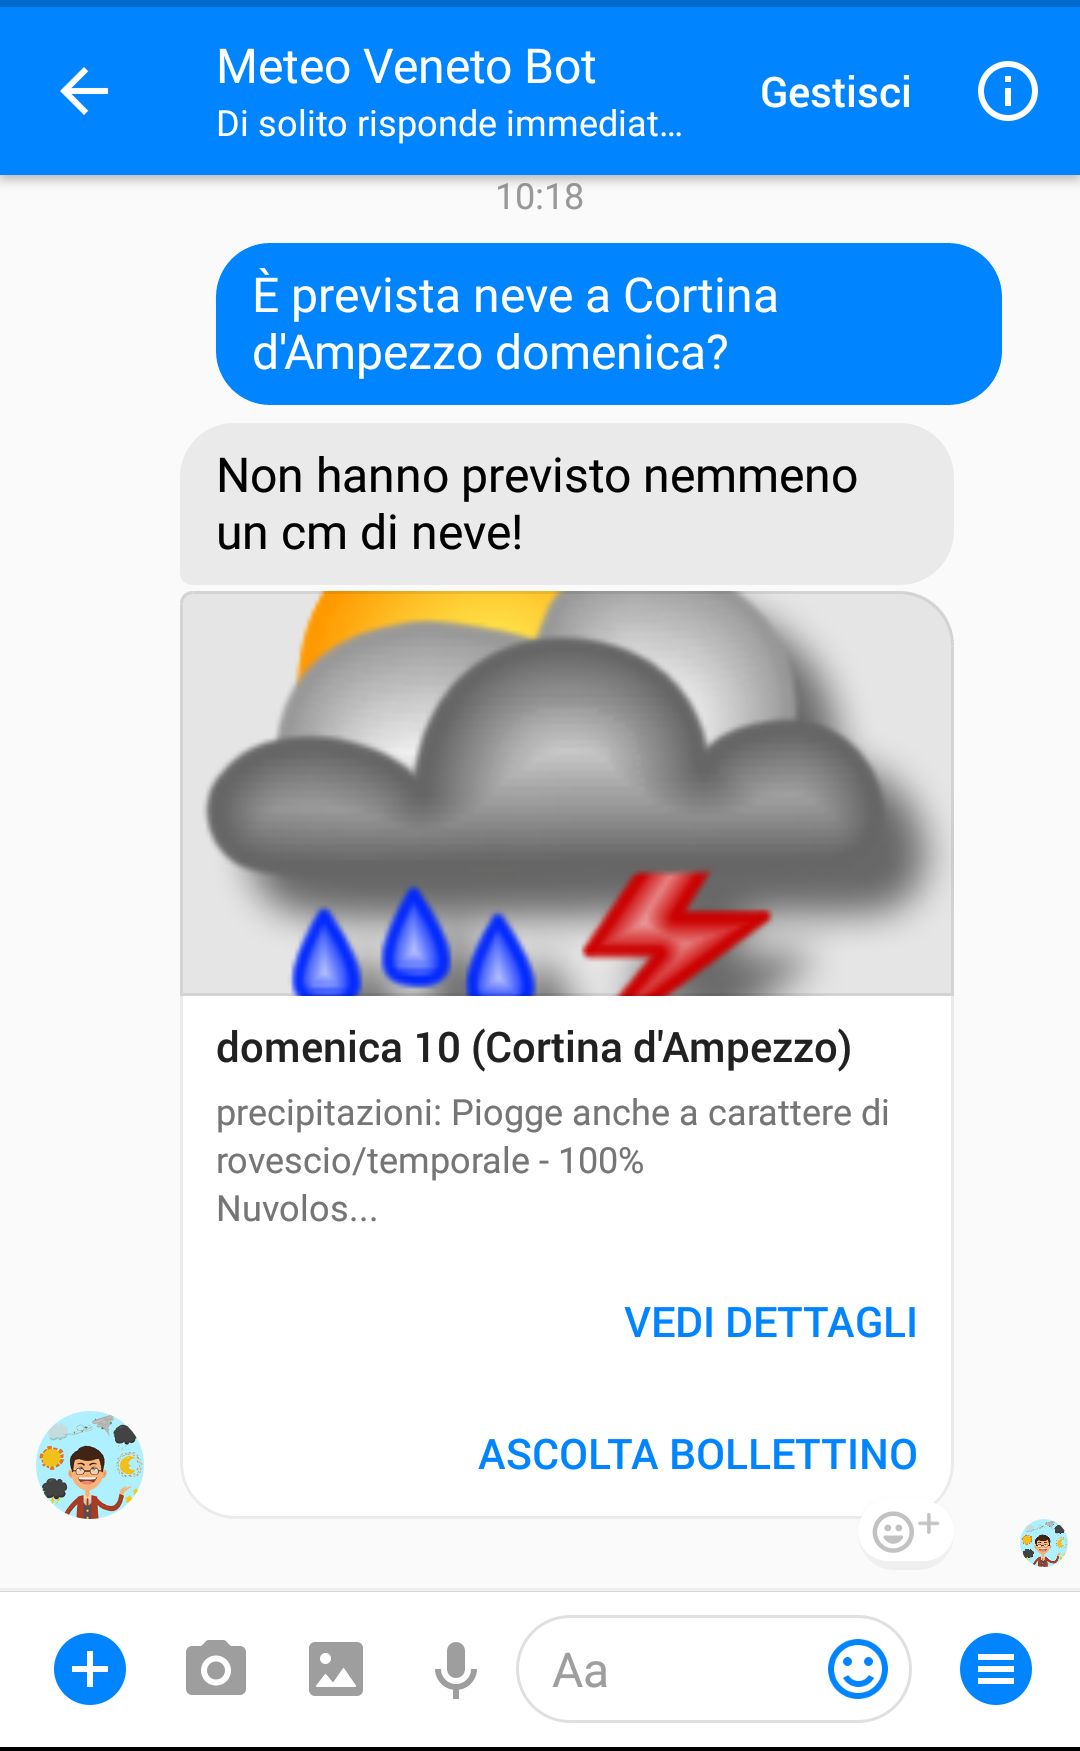
\includegraphics[scale=0.15]{../Immagini/neve.png}
		\caption{Esempio dell'intent richiesta\_neve}
	\end{figure}
	\item \textbf{richiesta\_bel\_tempo}: permette all'utente di chiedere se è previsto bel tempo in una specifica giornata o un periodo di tempo (es. weekend), in un determinato comune. La risposta è formata da due messaggi: il primo mostra le giornate dove è previsto bel tempo, tra quelle richieste dall'utente, il secondo contiene i caroselli delle previsioni.
	\begin{figure}[!h]
		\centering
		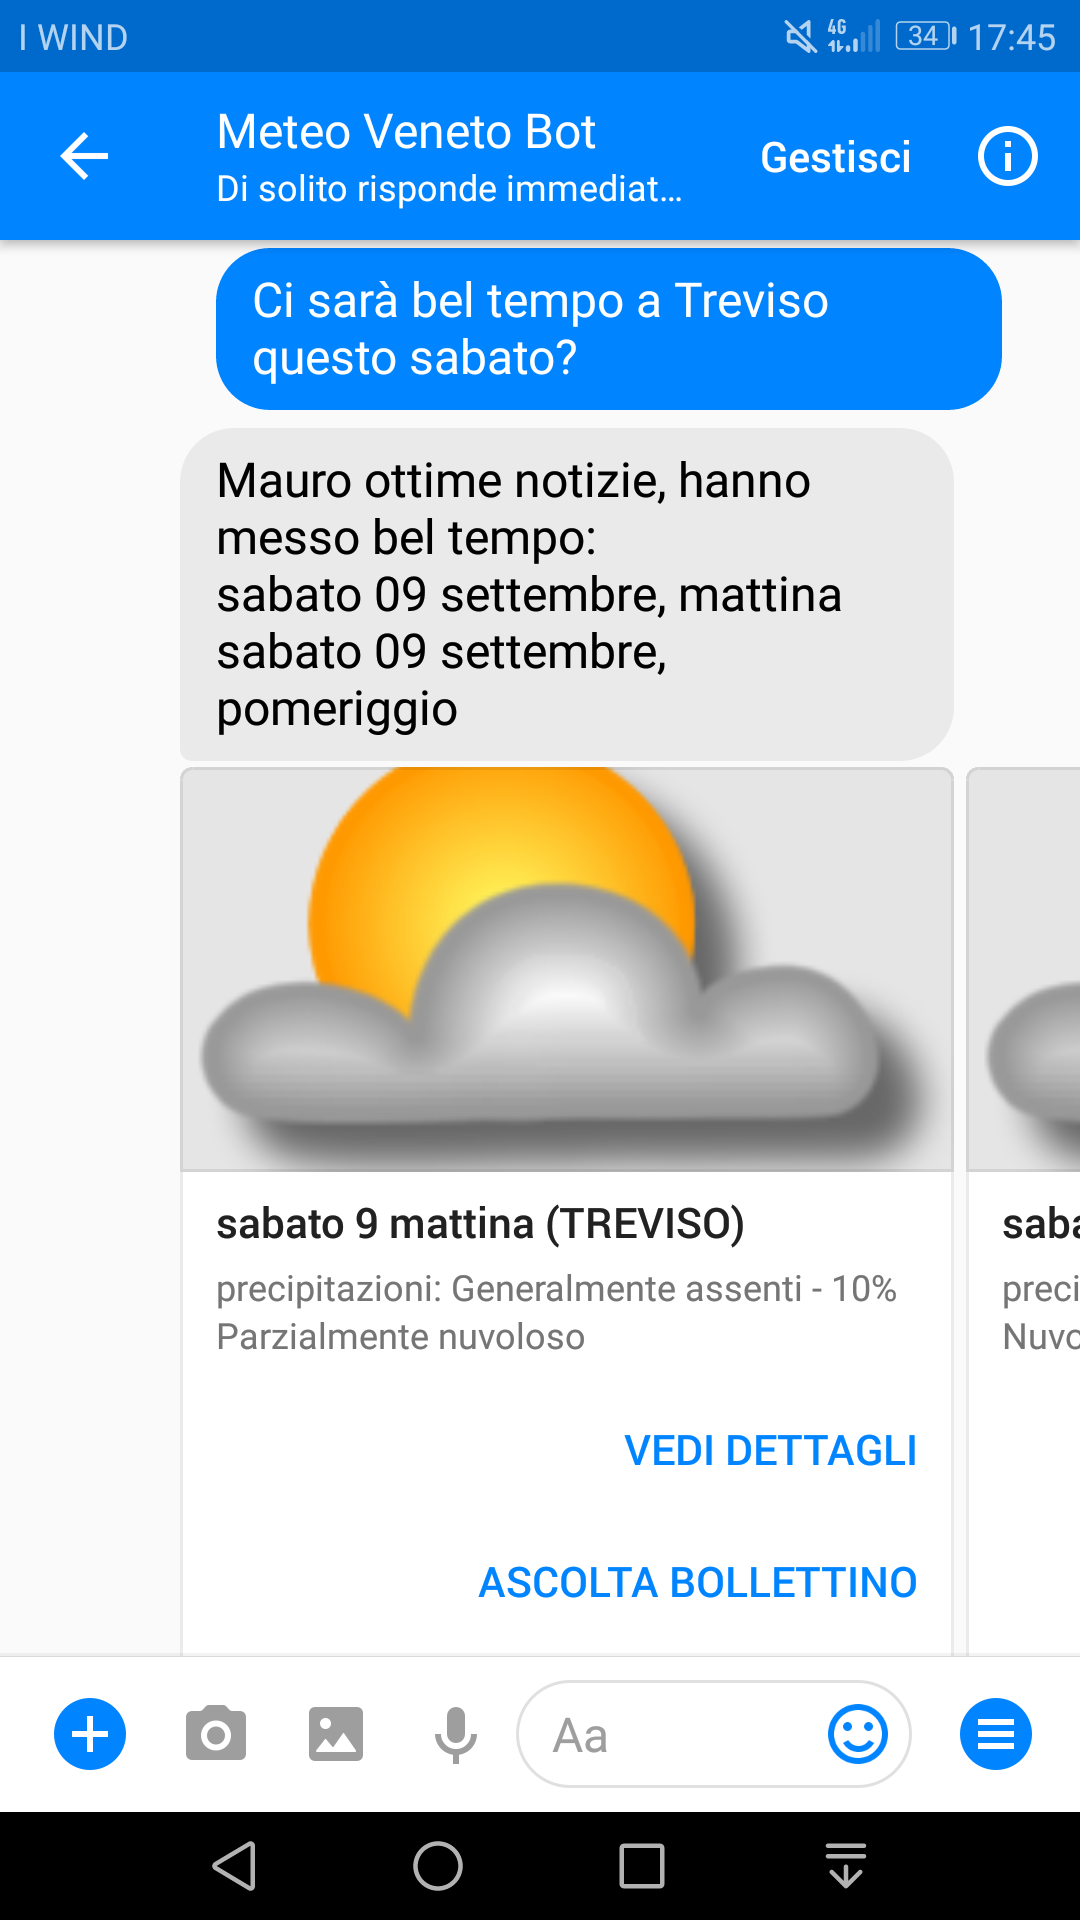
\includegraphics[scale=0.15]{../Immagini/richiesta_bel_tempo.png}
		\caption{Esempio dell'intent richiesta\_bel\_tempo}
	\end{figure}
	\item \textbf{richiesta\_brutto\_tempo}: permette all'utente di chiedere se è previsto brutto tempo in una specifica giornata o un periodo di tempo (es. weekend), in un determinato comune. La risposta è formata da due messaggi: il primo mostra le giornate dove è previsto brutto tempo, tra quelle richieste dall'utente, il secondo contiene i caroselli delle previsioni.
	\begin{figure}[!h]
		\centering
		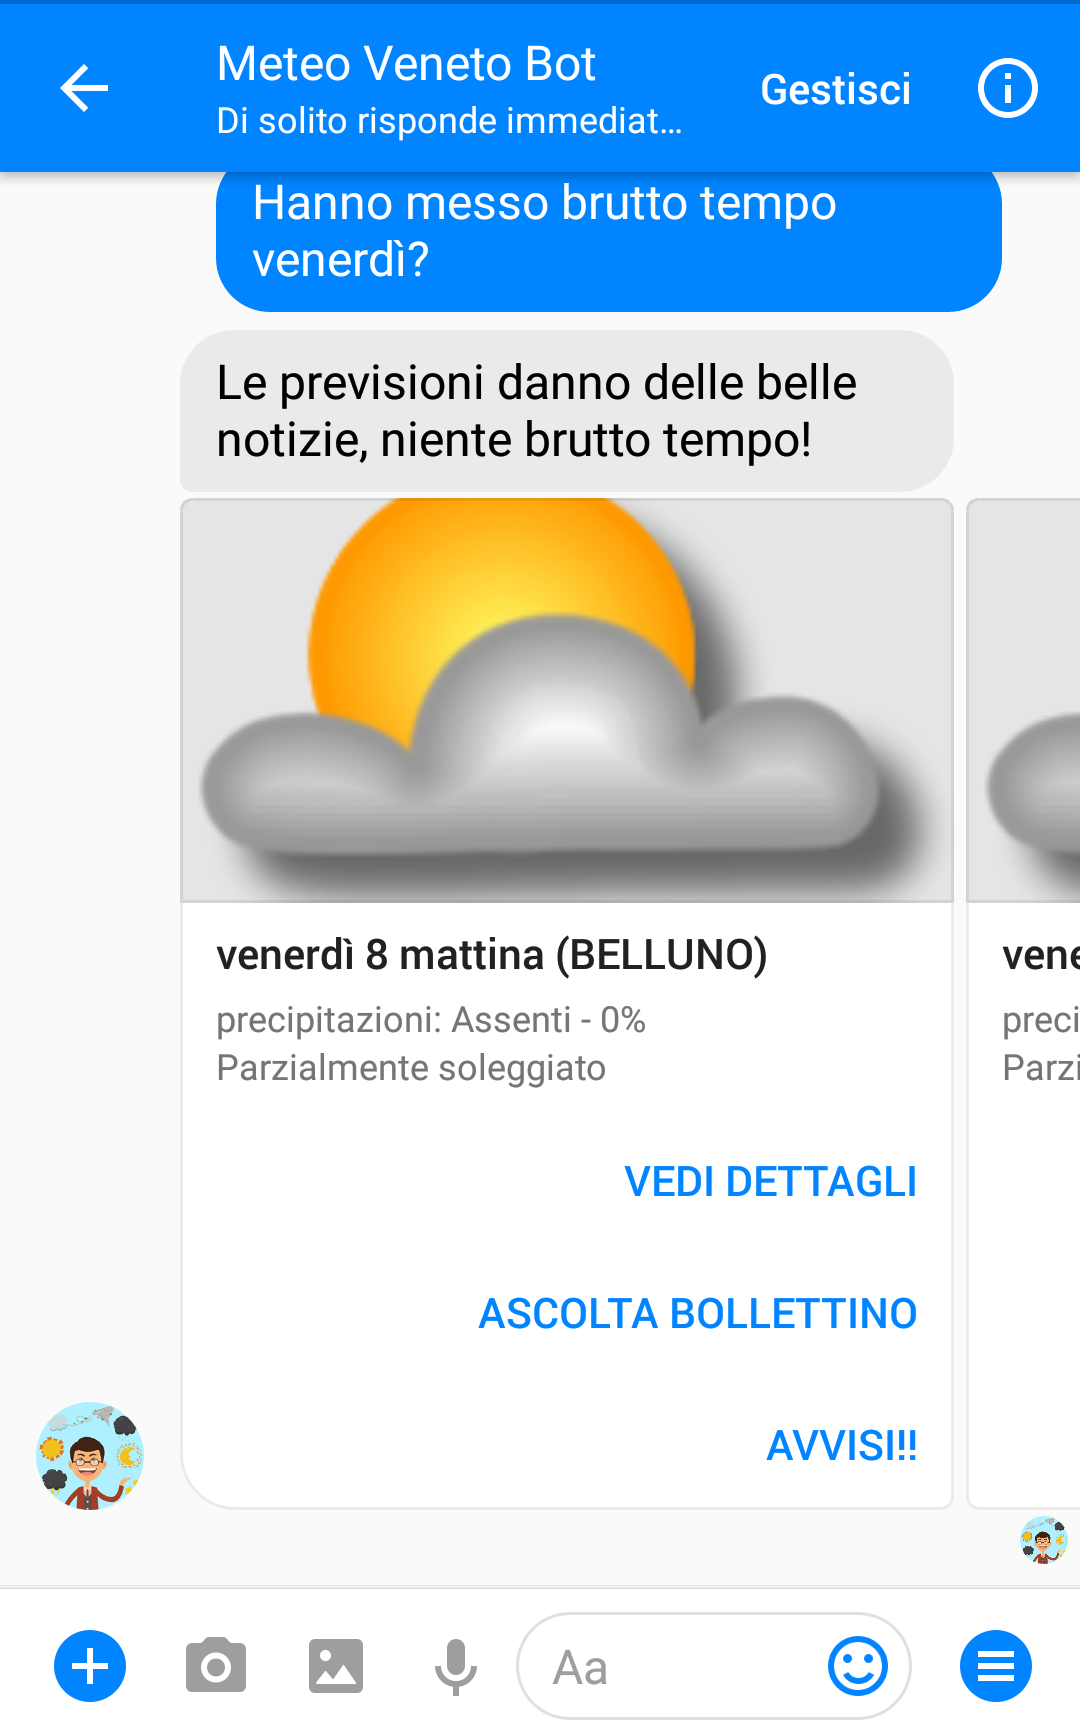
\includegraphics[scale=0.15]{../Immagini/richiesta_brutto_tempo.png}
		\caption{Esempio dell'intent richiesta\_brutto\_tempo}
	\end{figure}
	\item \textbf{richiesta\_temperature}: permette all'utente di chiedere le temperature previste in una specifica giornata o un periodo di tempo (es. weekend), in un determinato comune. La risposta contiene le temperature massimi e minime previste fornite da ARPA Veneto.
	\begin{figure}[!h]
		\centering
		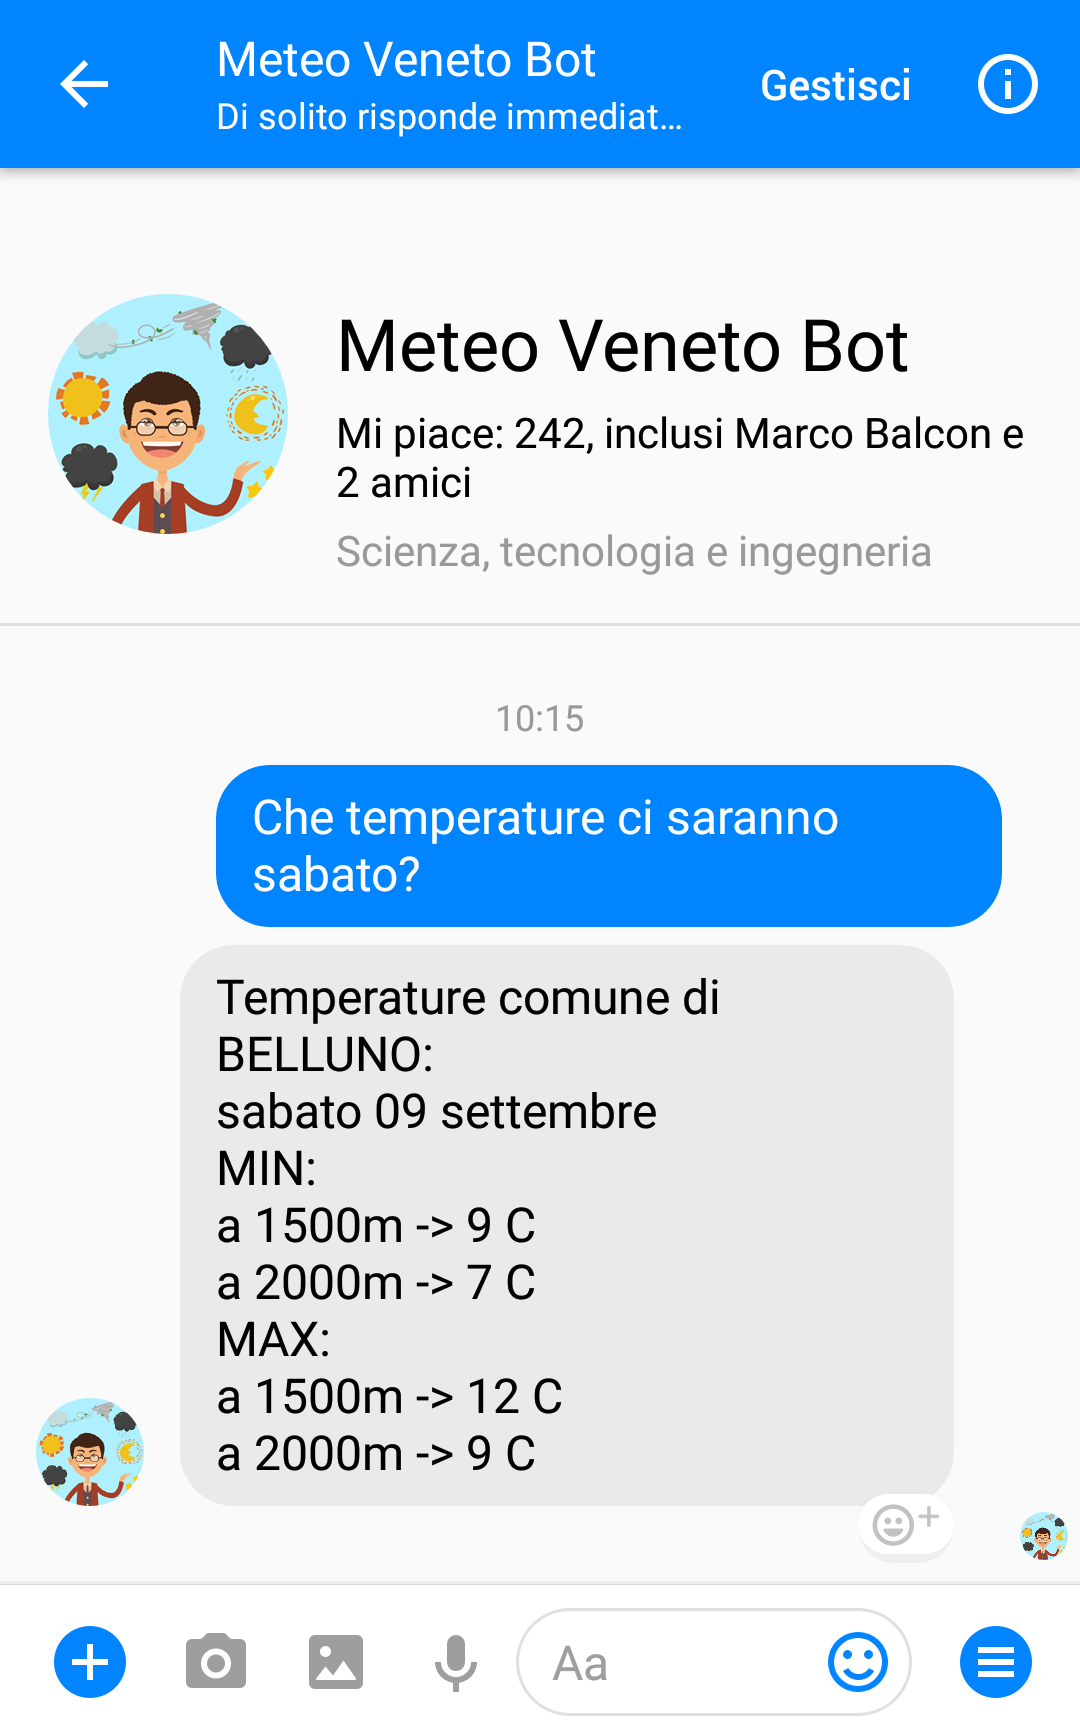
\includegraphics[scale=0.15]{../Immagini/temperature.png}
		\caption{Esempio dell'intent richiesta\_temperature}
	\end{figure}
	\item \textbf{ascolta\_bollettino}: permette all'utente di chiedere il bollettino audio emesso da ARPA Veneto ogni giorno. La risposta contiene il file audio richiesto.
	\begin{figure}[!h]
		\centering
		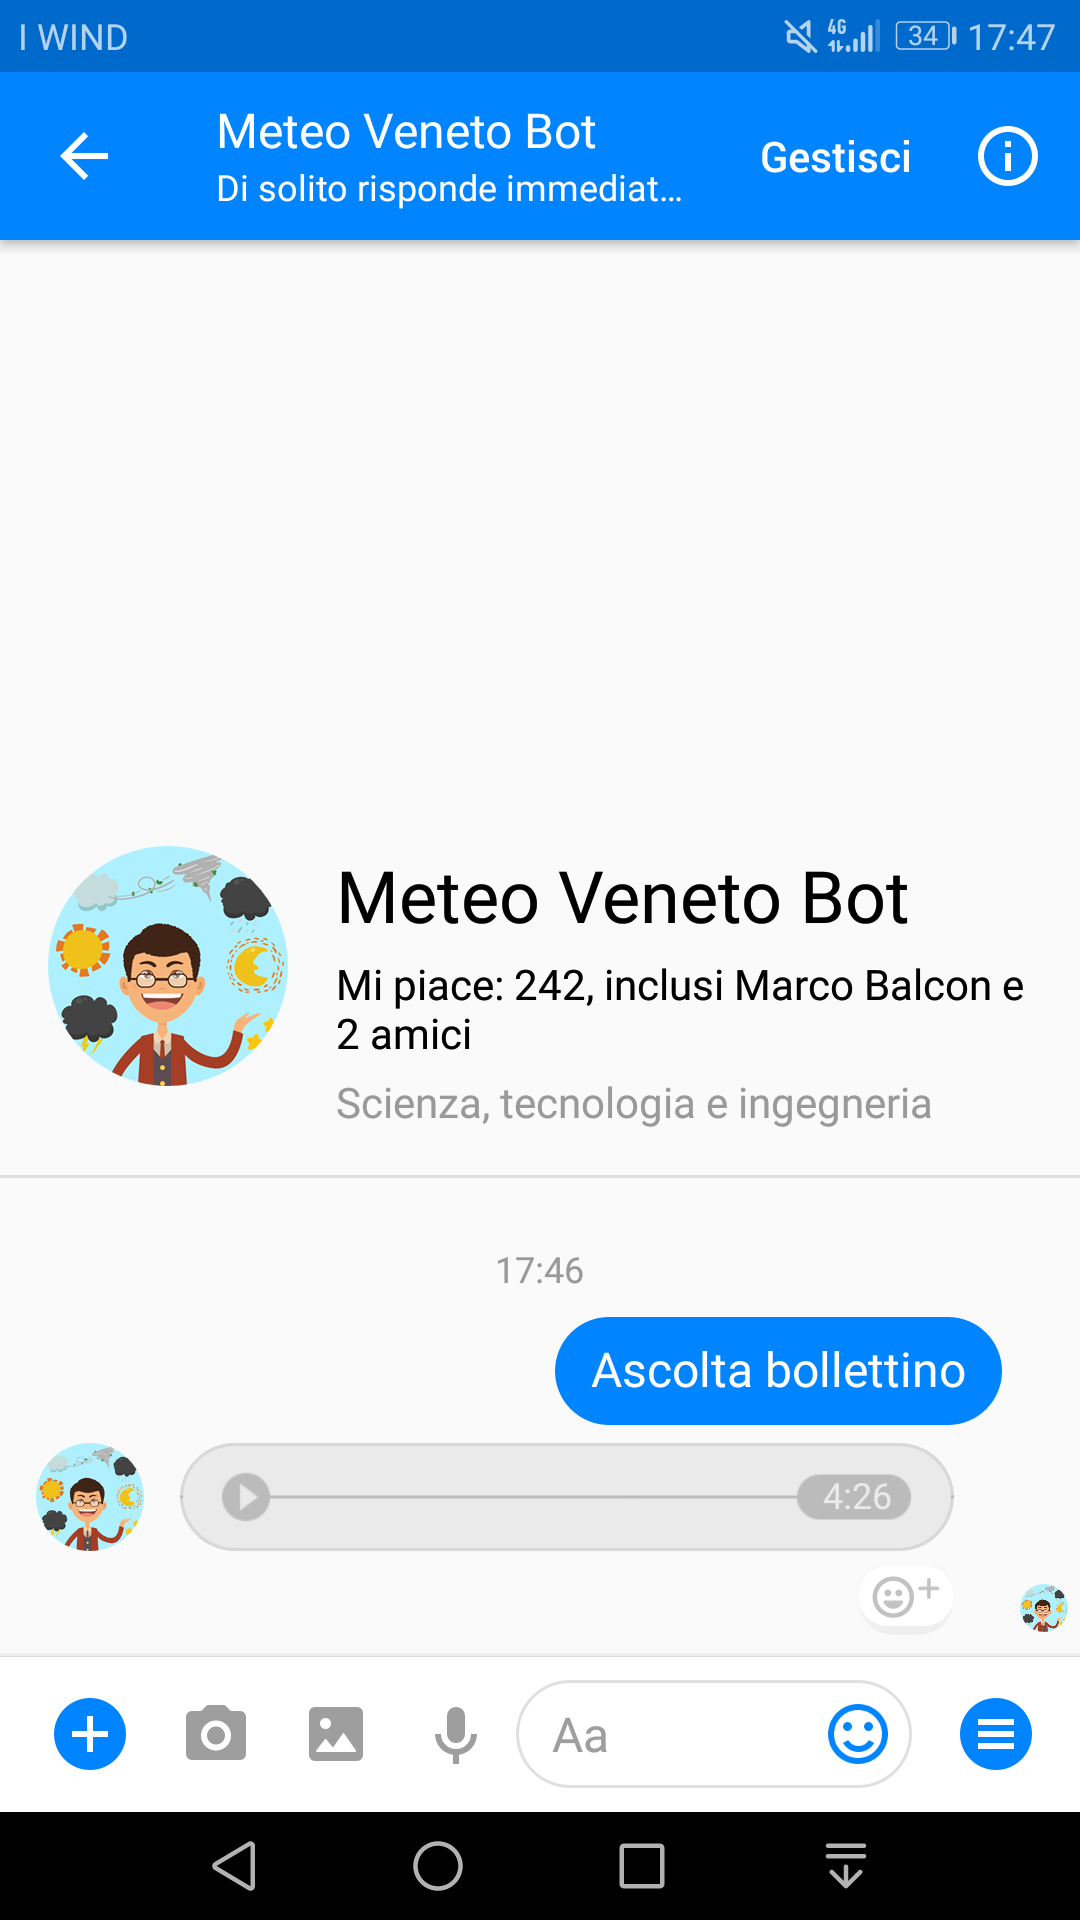
\includegraphics[scale=0.15]{../Immagini/bollettino.png}
		\caption{Esempio dell'intent ascolta\_bollettino}
	\end{figure}
\newpage
	\item \textbf{fenomeni\_particolari}: permette all'utente di chiedere se sono presenti avvisi o fenomeni particolari emessi da ARPAV. La risposta contiene questi avvisi, se presenti.
	\begin{figure}[!h]
		\centering
		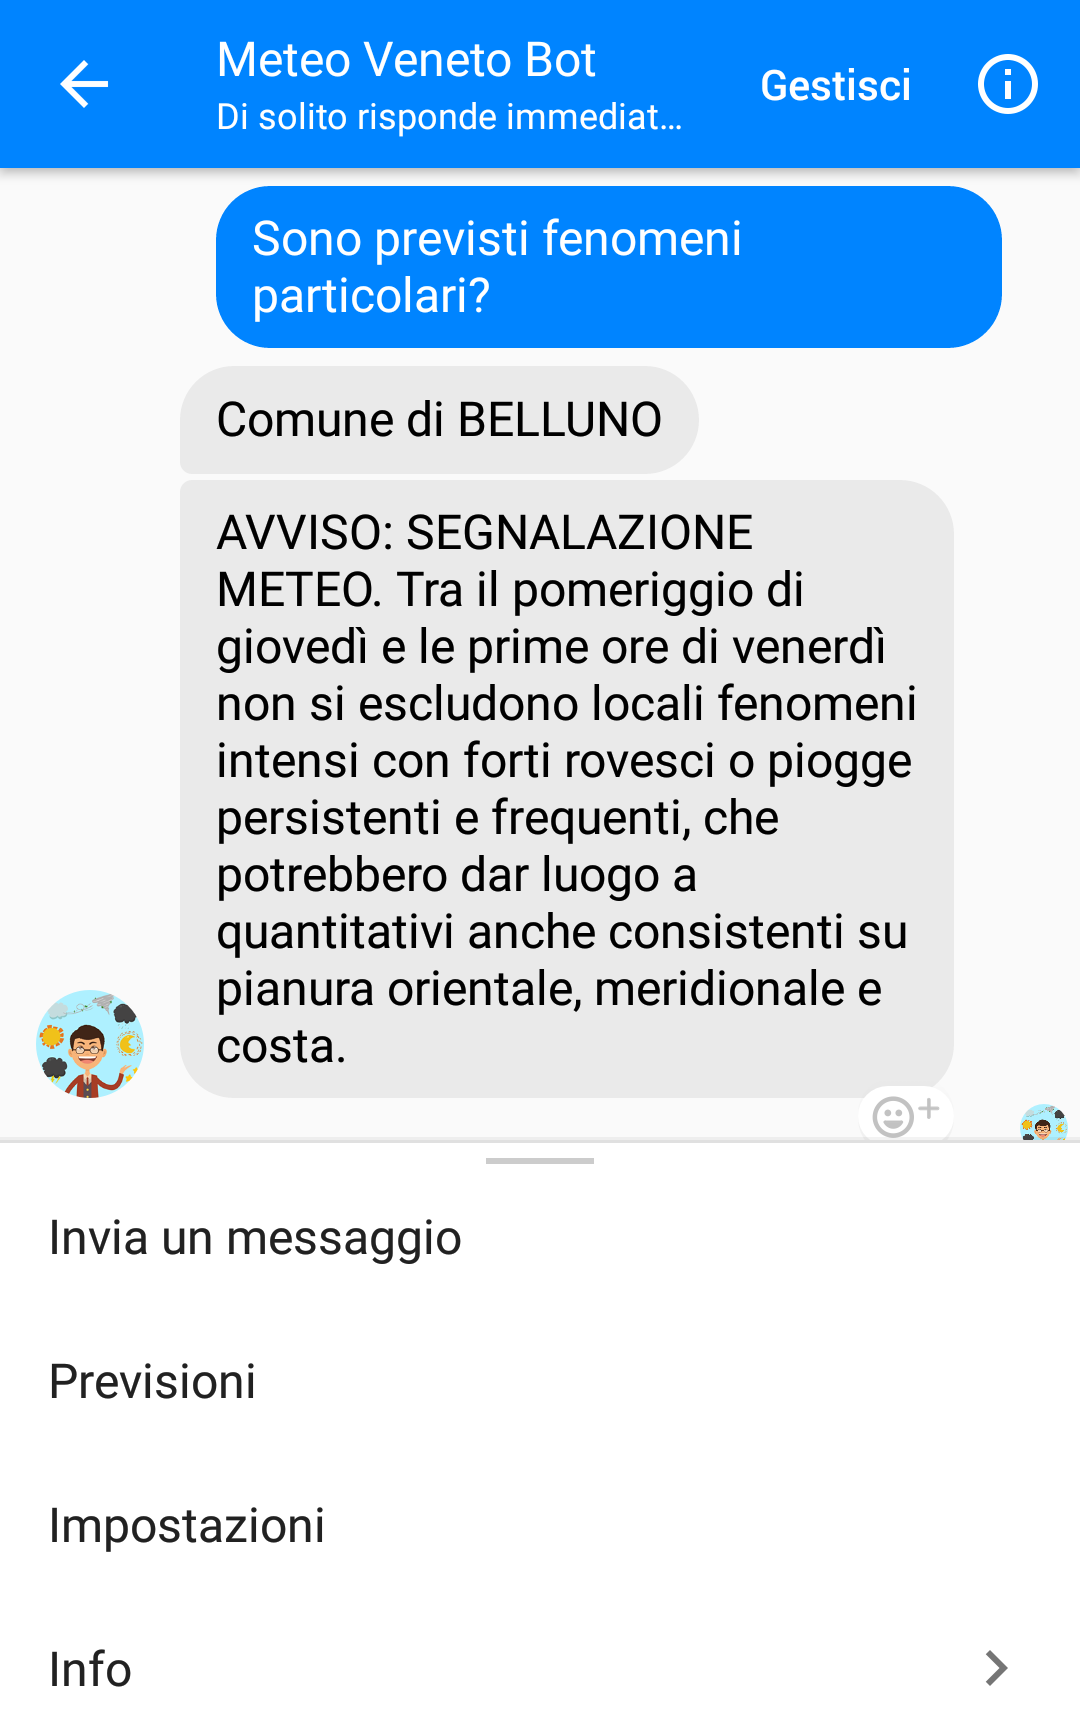
\includegraphics[scale=0.15]{../Immagini/fenomeni.png}
		\caption{Esempio dell'intent fenomeni\_particolari}
	\end{figure}

\end{itemize}

\subsubsection{Entity}
Nella progettazione di questo \emph{agent} ho creato queste nuove \emph{entities}:
\begin{itemize}
	\item \textbf{fenomeni atmosferici}: ho creato quattro \emph{entities} per \textbf{sole}, \textbf{pioggia}, \textbf{neve}, \textbf{nebbia}, in modo da gestire i possibili sinonimi che un utente può scrivere;
	\item \textbf{time}: si tratta di una \emph{composite entity} per gestire gli orari e le date scritte dall'utente. In particolare questa \emph{entity} combina tre \emph{system entity} fornite da api.ai:
	\begin{itemize}
		\item \textbf{@sys.date}: per le date in formato standard (es. 31 agosto);
		\item \textbf{@sys.date-period}: per un periodo di tempo formato da più giorni (es. weekend);
		\item \textbf{@sys.time-period}: per una parte del giorno (es. mattina, pomeriggio, notte);
	\end{itemize}
Combinando queste \emph{entities} l'utente può specificare precisamente le previsioni che desidera ricevere. Può infatti porre al \gls{Chatbot} domande del tipo: \emph{"Che tempo farà domani sera?"}, \emph{"Dimmi le previsioni per il prossimo weekend"}, \emph{"Ci sarà il sole venerdì pomeriggio?"}.
\end{itemize}
\begin{figure}[!h]
	\centering
	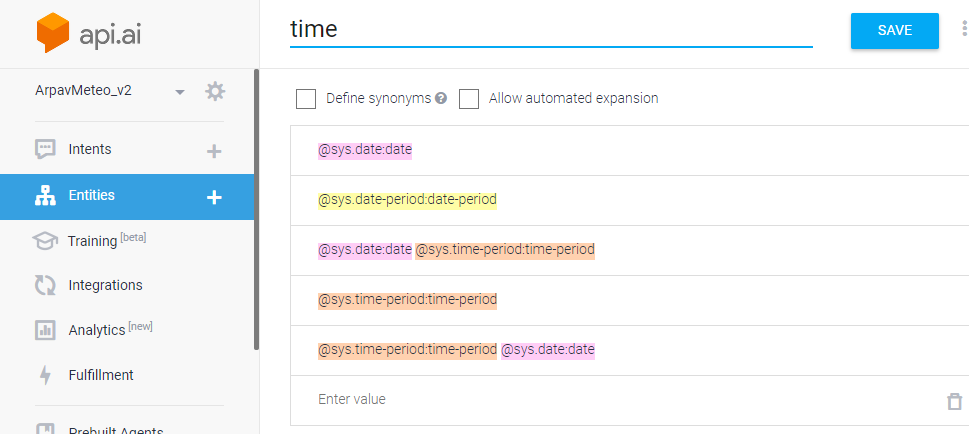
\includegraphics[scale=0.5]{../Immagini/time.png}
	\caption{Entity time definita nell'agent}
\end{figure}
\newpage
\section{Progettazione delle componenti}
Per quanto riguarda la progettazione delle componenti da aggiungere al software aziendale ho deciso di creare due classi per ciascun \gls{Chatbot}, con un comportamento simile. La prima ha il compito di:
\begin{itemize}
	\item \textbf{interrogare api.ai}, costruendo il messaggio da inviare con il token dell'agent, l'input e il sessionId dell'utente;
	\item \textbf{analizzare la risposta}, invocando il metodo corretto a seconda del valore del campo \emph{action} del \gls{JSON}.
\end{itemize}
La seconda classe invece contiene tutti i metodi che rappresentano la logica del \gls{Chatbot}, analizzando i \emph{parameters} del \gls{JSON} ritornato da api.ai e formulando la risposta da visualizzare nella chat. Questi metodi hanno riutilizzato dei componenti già presenti nel software, per costruire modelli di risposta già previsti nel \gls{Chatbot} prima del mio arrivo.


\section{Jaro Winkler distance}
Durante l'attività di progettazione mi sono reso conto come fosse necessario gestire un possibile errore di scrittura dell'utente in una delle sue domande, soprattutto nelle parole fondamentali per formulare le risposte, come ad esempio il nome di un comune per il \gls{Chatbot} del meteo o il nome di una conferenza in quello degli eventi. In un primo momento infatti l'input dell'utente veniva utilizzato direttamente nelle \emph{query} \gls{SQL} per interrogare il database ed ottenere i dati di interesse, soprattutto attraverso l'operatore \emph{"LIKE"}. In questo modo però non è possibile gestire il caso in cui un utente scriva ad esempio il comune "Padvoa", intendendo Padova. \\
Per ovviare a questo problema quindi è stato deciso di introdurre, dopo uno studio delle possibili soluzioni, la Jaro Winkler distance\footcite{jaro}, ossia una metrica che misura la "distanza" tra due stringhe per capire quanto esse siano simili tra loro. Grazie a questa accortezza, nel caso di errore di scrittura, il \gls{Chatbot} è in grado di:
\begin{itemize}
	\item fornire una serie di opzioni di cosa secondo lui l'utente voleva scrivere, dando la possibilità ad esso di selezionare quella giusta;
	\item fornire i dati richiesti dall'utente nel caso ci sia un'unica corrispondenza simile a quanto scritto dall'utente nel database.
\end{itemize}
\begin{figure}[!h]
	\centering
	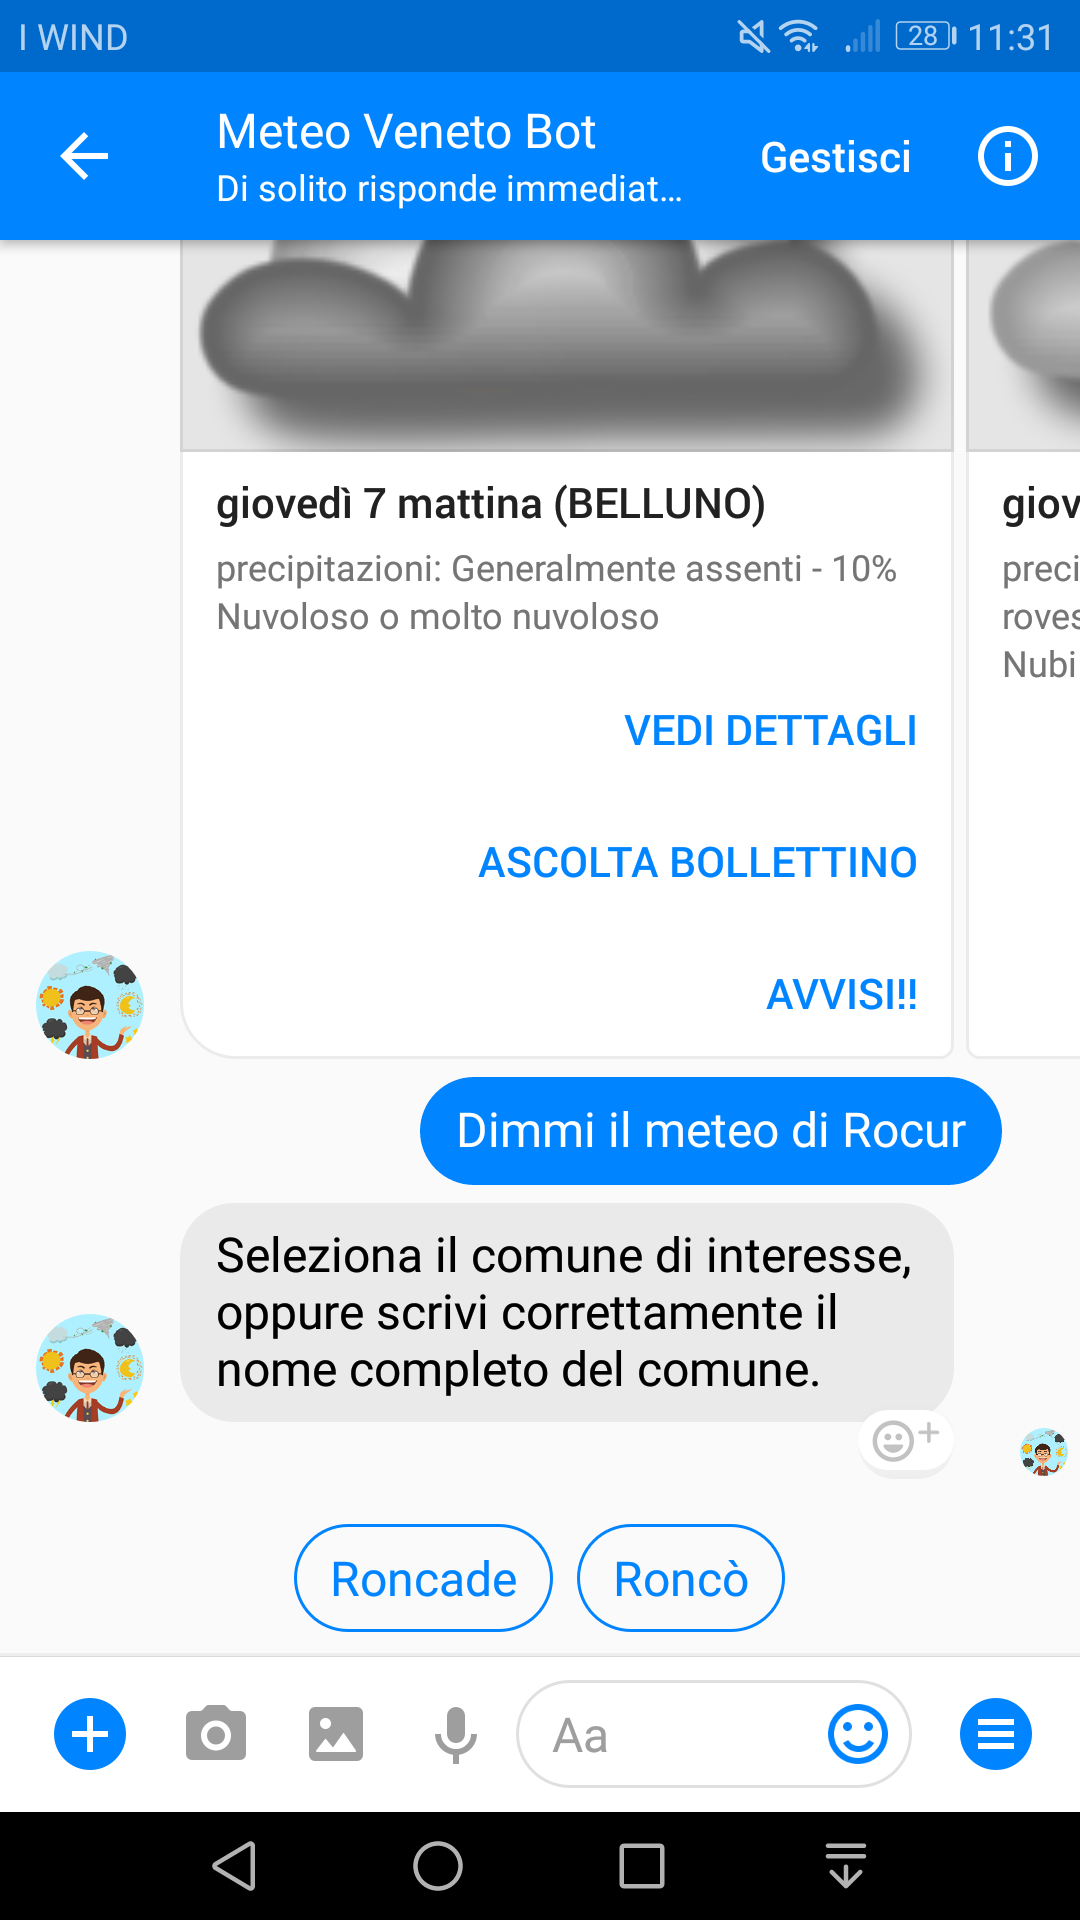
\includegraphics[scale=0.19]{../Immagini/meteo_scelta.png}
	\caption{Esempio di utilizzo della Jaro Winkler distance}
\end{figure}
